\documentclass[10pt,twocolumn]{article}
\usepackage{graphicx}
\usepackage{fancyhdr}
\usepackage{amssymb,amsmath}
\usepackage[usenames,dvipsnames]{color}
\usepackage[colorlinks,citecolor=RedViolet,urlcolor=blue]{hyperref}
\usepackage{doi}
\usepackage{setspace}
\usepackage[paperwidth=8.5in, paperheight=11in,top=1in, bottom=1in, left=1in, right=1in]{geometry}
\usepackage[compact]{titlesec}
\usepackage{abstract}
\usepackage[position=t,singlelinecheck=off,justification=raggedleft]{subcaption}
\usepackage[authoryear,square]{natbib}
\usepackage{aas_macros}
\pagestyle{fancy}
\fancyhead[R]{Veibell \thepage}
\fancyhead[L]{}

\newcommand{\vinote}[1]{\textcolor{red}{\textbf{#1}}} %If you want \inote{#} instead of just \note #, for inline notes
\def\vnote#1\par{\textcolor{red}{\textbf{#1}}\\} %Make note bold and red, re-add newline
\newcommand{\req}{\ensuremath{\rho_{eq}}}
\newcommand{\inote}[1]{\textcolor{blue}{\textbf{#1}}} %Inline notes in blue
\def\note#1\par{\textcolor{blue}{\textbf{#1}}\\} 

\begin{document}
\title{Relationship between solar wind, $D_{st}$, and plasmasphere trough mass density on one-hour time scales}
\author{
Victoir Veibell\footnote{vveibell@gmu.edu}
\and
R.S. Weigel\footnote{rweigel@gmu.edu}}


\setlength{\parskip}{3ex}
\renewcommand{\labelitemi}{$-$}
\titlespacing{\section}{0pc}{0.2pc}{-1pc}
\titlespacing{\subsection}{0pc}{0.1pc}{-1pc}
\titleformat*{\section}{\normalsize\bfseries}
\titleformat*{\subsection}{\small\bfseries}

\twocolumn[
  \begin{@twocolumnfalse}
\maketitle
\hrule
\begin{abstract}
This paper compares various magnetosphere conditions around the onset of geomagnetic events, defined as decreases in $D_{st}$ below a threshold value or $\rho_{eq}$ above a threshold value. 

\vnote More detail

%It confirms results from previous papers that a sudden drop in $D_{st}$ correlates with a spike in equatorial mass density under certain conditions, while adding a level of depth and specification to the applicability of their results. It compares data at 1-hour averages to data at 1-day averages to examine if the trend holds at varying time scales and finds that it does, so long as the data is pre-processed to linearly remove a large time scale $F_{10.7}$ dependence. By then looking at an hourly average of parameters from 24 hours before event onset to 48 hours after, short timescale trends can be discerned.

\vspace{2em}
\end{abstract}
 \end{@twocolumnfalse}
  ]

\saythanks

\section{Introduction}

The plasma trough is the transition region between the high density and low temperature plasmasphere and the lower density and, in the equatorial plane, higher energy magnetosphere \citep{Mayr1968ModelMagnetosphereTemperature}.  Although there are well--validated models of the plasmasphere density as a function of $L$ (\cite{Gallagher1988EmpiricalModelPlasmasphere}, \cite{LemaireEarthsPlasmasphere}, \cite{Takahashi2006}, and \cite{Takahashi2010}) and plasmapause boundaries (\cite{LemaireEarthsPlasmasphere}, \cite{Moldwin2002ModelPlasmapause}, \cite{OBrien2003EmpiricalPlasmapause}), the dependence of the plasma trough on solar wind conditions has not been extensively studied.

\cite{Gallagher1988EmpiricalModelPlasmasphere} modeled the the plasmasphere as a simple linear fit dependent on $L$ shell, geographic altitude, geomagnetic latitude, and $K_p$.  \inote{What was major finding?} \cite{Hamilton1988RingCurrentDevelopment} analyzed a strong geomagnetic storm and compared energy measurements of the ring current to $D_{st}$, along with measurements of ring current compositions before, during, and after the storm.  \inote{What did they find/conclude?}

\cite{Lotoaniu1999PlasmaMassDensity} used measurements from the \inote{???} instrument on the CRRES sateelite and compared in-situ measured plasma mass density to that inferred by ground-based ULF wave measurements that extended to the plasmatrough.  \inote{What did they find/conclude?}

\cite{Takahashi2006} estimated magnetospheric mass density using measurements from the CRRES satellite during a 73-day period in 1991 and found that the average ion mass, $M=\rho/n_e$, correlated with geomagnetic activity, with more negative $D_{st}$ values corresponding to slightly higher average ion mass densities.  They also found a relationship between the average ion mass and 1.5- and 3-day averages of $K_p$, with an increasing correlation as $K_p$ was smoothed to longer timescales.  The CRRES measurements used occurred in the MLT range of 12:00 and 18:00 mostly in the plasma trough (between 2-7$R_E$) on an elliptical, nearly equatorial orbit.

\cite{Denton2006} showed a relationship between $D_{st}$ and the field line distribution of plasma density, and specifically along the same field lines as looked at in later papers (6-8$R_E$). They found that the distribution depends on $L$,.

\cite{Takahashi2010} developed a mass density dataset using measurements from the SEM \inote{Check instrument} instruments on the GOES satellites from 1980 through 1992, with most measurements in the range $L=6.8\pm0.2 R_E$. The mass density $\rho$ was estimated using the the Alf\v'en wave velocity relationship, $V_A=B/\sqrt{\mu_0\rho}$, a magnetic field model, and a numerical solution to a wave equation with an ionospheric boundary and the assumption of a zero resistance ionosphere.  The equatorial mass density, $\rho_{eq}$, was derived from the estimated mass density using a power law dependence on the geocentric distance to the field line of the observation, $R$, $\rho=\rho_{eq}L/(R/R_E)$. 

\cite{Takahashi2010} noted that downward spikes in the $D_{st}$ index coincided with with significant changes in $\rho_{eq}$ at for $L$ near 6.8~$R_E$. For five storms, two had $\rho_{eq}$ spikes after the $D_{st}$ drop, two had $\rho_{eq}$ spikes before the drop, and one showed little change in $\rho_{eq}$.  A key result was that when daily-averaged measurements were considered, an enhancment in $\rho_{eq}$ appeared on the same day as minimum $D_{st}$, indicating the possibility of a solar wind control over $\rho_{eq}$.

The results of \cite{Takahashi2006} and \cite{Takahashi2010} are consistent with other results on changes in mass density in the plasma trough region.  \cite{Yao2008} studied the relationship between $D_{st}$ and ion number density for different ion species in different regions (ring current and plasma sheet) and found a general correlation during each of the four storms considered.

In this work we consider the dependence of plasmaspheric mass density in the \cite{Takahashi2010} in more detail in an attempt to identify the solar wind processes that drives changes in the plasma trough density.

\section{Data Preparation}

The parameters $\rho_{eq}$ and $F_{10.7}$ used in this work are from the dataset associated with \cite{Denton}, with data available from 1980 through 1991; all other parameters are from \cite{Reconstruction} from 1972 through 2013, which are on a 1--hour time grid. $\rho_{eq}$ is the inferred equatorial mass density based on the 3rd harmonic torodial frequency of magnetic field measurements.  The smallest cadence for $\rho_{eq}$ values is 10 minutes.  To compute an hourly average over the same interval for which the solar wind parameters were averaged, the median of all $\rho_{eq}$ values in a given hourly range was used.  Fill (NaN) values were used for hours in which no measurements were available.  In cases where $\rho_{eq}$ was available from multiple Geostationary Operational Environmental Satellites (GOES) satellites at the same time in the \cite{Denton} dataset, the value from GOES 6 was selected.  In the dataset, measurements from GOES 6 had the longest time span of coverage.  An overview of the data is shown in Figure~\ref{AllData}.

In this work, events defined to occur when $D_{st}$ or $\rho_{eq}$ crosses a threshold value, as indicated in by horizontal dashed lines in the respective panels of Figure~\ref{AllData}.  In finding $\rho_{eq}$ events, all fill values were replaced with linearly interpolated values. 

Figure \ref{AllData} shows values of solar wind averages and mass density from GOES 6.  The corresponding 27-day correlations for GOES 2, 5, and 7 are 0.81, 0.78, and 0.87, and the time range of coverage of measurements from these satellites are 1980-01-01/1983-05-16, 1983-01-01/1987-02-28, and 1983-05-27/1991-08-29

Figure~\ref{ccplot} shows the long-term trends of GOES 6 based $log(\rho_{eq})$ and $F_{10.7}$ computed using the median values in 27-day (non-overalpping?) windows using all non--fill hourly values.  A scatter plot of these two lines is shown in Figure~\ref{ccplot}.  The linear correlation is found to be $0.94$ matching the value found by \cite{Takahashi2010} who used measurements from all satellites in the time interval of 1980 through 1991.  

\section{Results}

\subsection{$D_{st}$ and $\rho_{eq}$ Events}

Two types of events are considered. The first is a drop in $D_{st}$ below the threshold of $-50$~nT.  The second is an increase in $\rho_{eq}$ above 40~amu/cm$^3$.

Our first analysis uses data only from the time interval 1989-1991. For both types of events, the hour of the threshold crossing defines the zero epoch time, and for each event $8\cdot24$ hours were kept after each event and $4\cdot24$ hours before each event.  To compute the epoch averages on a daily time scale, the median value of all measurements for all events centered on a window of $\pm 12$ hours was computed, and these windows were shifted in increments of $24$~hours. (Similar results are obtained if we first reduce each event time series to have a 1-day cadence by computing medians in 1-day bins and then compute the medians accross events.)  Error bars for each parameter were computed using the standard deviation of the number of values used in computing the median divided by the square root of the number of values used.

In the upper panel of \ref{DailyAverages}, $D_{st}$ events are shown.  The minimum $D_{st}$ median is $-48$~nT.  Consistent with \cite{Takahashi2010}, $D_{st}$ events correspond to elevated $\rho_{eq}$, although the magnitude of increase observed here is $\sim 2$ amu/cm$^3$ instead of the value of $\sim 10$ amu/cm$^3$ found in \cite{Takahashi2010}.  The vertical green bars in the $\rho_{eq}$ plot show the number of $\rho_{eq}$ values that were used to compute its median and error bars.  Note that for $D_{st}$, the number of measurements used in computing the medians is much larger as we use all available $D_{st}$ measurements instead of restricting to only values where a non--fill $\rho_{eq}$ value existed.  

In the lower panel of \ref{DailyAverages} it is shown that all trends seen in the analysis of 1989-1991 also hold for the entire run of GOES 6 over 1983-1991, including the magnitude of change in $\rho_{eq}$ across event onset.

It was found that $\rho_{eq}$ enhancements do not clearly correspond to a signature in $D_{st}$, but that there is a trend for such enhancements to occur when $B_{z}$ in the IMF is positive.  This is consistent with \cite{Takahashi2010} who note that very large increases in $\rho_{eq}$ often corresponded to movement of the plasmasphere to beyond geosynchronous distances. 

This method finds 669 such periods between May 1983 and August 1991 with an average duration of 9 hours and a median duration of 3 hours. Figure \ref{Storms} shows the average values of all events over a window of 24 hours before onset and 48 hours after. Figure \ref{Storms}a shows events selected by looking for event onsets where $D_{st}$ crossed a threshold of $-40$~nT. The dashed red lines indicate plus and minus one standard deviation of values from all events that went into the average. The final plot in the stack shows both $\rho_{eq}$ and a bar plot of how many valid data points went into the $\rho_{eq}$ average. Since $\rho_{eq}$ comes from a sparser dataset, it has less valid points contributing to the averages than the other parameters in the stack. A subset of longer duration events will be looked at later. 

This figure shows a definite spike in the $Z$ component of the magnetic field, as well as the defined drop in $D_{st}$, but no obvious change in mass density at an hourly timescale. This points to an issue with only looking at long-timescale trends between density and $D_{st}$, and allows for the possibility that other factors are influencing the long term correlation since there's no obvious connection on a short timescale. One possibility is that, as suggested in \cite{Takahashi2010}, $F_{10.7}$ plays a significant role in driving long term density values which biases the long term correlation of density and $D_{st}$.

Two types of events are considered. The first is a drop in $D_{st}$ below the threshold of $-40$~nT.  The second is an increase in $\rho_{eq}$ above $40$~amu/cm$^3$.

Our first analysis uses data only from the time interval 1989-1991.  In this interval, there were (?) $D_{st}$ events and (?) $\rho_{eq}$ events.  For both types of events, the hour of the threshold crossing defines the zero epoch time, and for each event $8\cdot24$ hours were kept after each event and $4\cdot24$ hours before each event.  To compute the epoch averages on a daily time scale, the median value of all measurements for all events centered window of $\pm 12$ hours was computed, and these windows were shifted in increments of $24$~hours. (Similar results are obtained if we first reduce each event time series to have a 1-day cadence by computing medians in 1-day bins and then compute the medians accross events.)  Error bars for each parameter were computed using the standard deviation of values used in computing the median dividied by the square root of the number of values used.

In the upper panel of \ref{DailyAverages}, $D_{st}$ events are shown.  The minimum $D_{st}$ median is $-48$~nT.  Consistent with \cite{Takahashi2010}, $D_{st}$ events corrspond to elevated $\rho_{eq}$, although the magnitude of increase observed here is on the order of $\sim2$~amu/cm$^3$ instead of $\sim10$~amu/cm$^3$ found in \cite{Takahashi2010}.  The vertical green bars in the $\rho_{eq}$ plot show the number of $\rho_{eq}$ values that were used to compute its median and error bars.  Note that for $D_{st}$, the number of measurements used in computing the medians is much larger as we use all available $D_{st}$ measurements instead of restricting to only values where a non-fill $\rho_{eq}$ value existed.  

In the lower panel of \ref{DailyAverages}, $\rho_{eq}$ events are shown.  Here we see that $\rho_{eq}$ enhancements do not clearly correspond to a signature in $D_{st}$, but that there is a trend for such enhancments to occur when $B_{z}$ in the IMF is positive.  This is consistent with \cite{Takahashi2010} who note that very large increases in $\rho_{eq}$ often corresponded to movement of the plasmasphere to beyond geosynchronous distances. 

A total of 668 events were found in the interval of May 1983 through August 1991 with an average duration of 9 hours and a median duration of 3 hours. Figure \ref{Storms} shows the average values of all events over a window of 24 hours before onset and 48 hours after. Figure \ref{Storms}a shows events selected by looking for event onsets where $D_{st}$ crossed a threshold of $-50$~nT. The dashed red lines indicate plus and minus one standard deviation of values from all events that went into the average. The final plot in the stack shows both $\rho_{eq}$ and a bar plot of how many valid data points went into the $\rho_{eq}$ average. Since $\rho_{eq}$ comes from a sparser dataset, it has less valid points contributing to the averages than the other parameters in the stack. A subset of longer duration events will be looked at later. 

This figure shows a definite spike in the $Z$ component of the magnetic field, as well as the defined drop in $D_{st}$, but no obvious change in mass density at an hourly timescale. This points to an issue with only looking at long-timescale trends between density and $D_{st}$, and allows for the possibility that other factors are influencing the long term correlation since there's no obvious connection on a short timescale. One possibility is that, as suggested in \cite{Takahashi2010}, $F_{10.7}$ plays a significant role in driving long term density values which biases the long term correlation of density and $D_{st}$.

\section{More specific events}
It's hypothesized that progressively picking more specific event criteria will allow for the possibility of more significant results, at the expense of more bias in the selection process and potentially less overall usefulness of the results. That said, the predictability of extreme events is of definite interest, so an attempt has been made to find some reproducible method of prediction. Looking at events that last longer than 12 hours and events with an onset threshhold less than $-80$nT finds both result in a spike in mass density, but also a definite lack of data availability to the point where that spike may be coming from less than five of the total 211 events. 

\subsection{Change in $\rho_{eq}$}
Instead of looking for events based on a threshold of $D_{st}$, we instead looked for a certain amount of change in $\rho_{eq}$ as the basis for event onset. Both raw change and percent change were done in case of bias towards high or low $\rho_{eq}$ periods, respectively, but neither showed any correlation to a change in $D_{st}$. 

\section{F10.7 dependence}
In an effort to analyze the dependence of $\rho_{eq}$ on $F_{10.7}$, a few tests were performed. \cite{Takahashi2010} mention a strong correlation between the two. The long term correlation could be a bias for $D_{st}$'s effects, so a linear model was created, recreating mass density purely from $F_{10.7}$ in the form of $\rho_{eq}(t)=a\cdot F_{10.7}(t)$. This re-created $\rho_{eq}$ shows around a 45\% correlation with the actual $\rho_{eq}$, suggesting a strong influence, while doing the same procedure with $D_{st}$ shows only a 20-25\% correlation. 

Figure \ref{f107bin} takes the events and bins them by the value of $F_{10.7}$ at event onset, then looks at both $\rho_{eq}$ and $B_z$. Error bars calculated in the same manner as before are added to the highest and lowest bins. A significant difference is seen in $\rho_{eq}$ between events taking place during periods of high $F_{10.7}$ and low $F_{10.7}$, while a much less significant, but still noticeable, difference is seen in $B_z$. Also of interest is how $\rho_{eq}$ only sharply reacts to $D_{st}$ events during periods of high $F_{10.7}$. The positive relationship seen in \cite{Takahashi2010} could be due to the short time period looked at, and that it coincides with periods of higher $F_{10.7}$.

Looking at GOES 2,5,6, and 7 shows that this post-onset $D_{st}$ spike happens in almost every case for periods of high $F_{10.7}$. Creating a linear model directly relating variables (and combinations of variables) to $\rho_{eq}$ also shows that $F_{10.7}$ most often has the highest correlation with $\rho_{eq}$. A sample of these correlations is shown in Table \ref{perltable}. The correlations were made by training a one-input linear model of 5-hour post-onset medians of each variable (or variables) against the median of $\rho_{eq}$ at, and four hours after, event onset. This was done by randomly sampling half of the data, generating the model, and testing against the other half, doing this process 100 times and then taking the median correlations.


\begin{table}[h]
\small
\begin{tabular}{|l|llll|}
\hline
 & GOES 2 & GOES 5 & GOES 6 & GOES 7\\ \hline
doy & -0.08 & +0.10 & -0.05 & +0.06 \\
MLT & -0.09 & -0.09 & -0.04 & -0.05 \\
Bz & +0.17 & -0.12 & +0.08 & -0.08 \\
Vsw & -0.04 & +0.29 & +0.06 & -0.06 \\
Dst & +0.27 & +0.66 & +0.06 & +0.22 \\
Rhosw & +0.34 & +0.63 & +0.07 & +0.34 \\
F107 & +0.42 & +0.14 & +0.49 & +0.42 \\
Bz+Vsw & +0.09 & +0.19 & +0.12 & -0.11 \\
Dst+F107 & +0.45 & +0.69 & +0.53 & +0.47 \\
All & -0.10 & +0.34 & +0.61 & +0.39 \\
\hline
\end{tabular}
\caption{Table of linear model correlations showing the median of 100 random samples. Each sample trained on half of the data (via randomly selected rows of the least squares matrix) and tested on the other half} 
\label{perltable}
\end{table}


\section{Appendix}
\subsection{Bias}
While attempting to reproduce Figure 11 from \cite{Takahashi2010}, an ambiguity in data-handling was found. It is unknown how they got from hourly $\rho_{eq}$ to daily medians, whether in one step or two steps, and whether the hourly medians are an hour ahead of each hour grid point, or a median of points a half hour to either side, so attempts were made to reproduce all possibilities and compare in order to find a data-handling method with the least bias. These attempts are shown in Figure \ref{blockmedian}. This also shows the effect of only considering events with a minimum before noon. All show a similar spike in $\rho_{eq}$ at the time of $D_{st}$ minimum, though none quite reproduce the exact values seen in \cite{Takahashi2010}. Figure \ref{allstorms} shows where the median falls for all of the found events during that period, as a sanity check for why the prior work would get median values nearing $30$~amu/cm$^3$. Both authors of this paper conducted independent trials to confirm that the data and analysis don't quite yield the results of Figure 11 in \cite{Takahashi2010} with the processes described in that paper, but the same general trend is still seen. 

To check for potential bias in the data as used by our analysis, we checked how the data availability varied with hour, shown in Figure \ref{nanperhour}. We also looked at how storm conditions affected data availability. Both a two sample t-test for difference in means and a Wilcoxon rank sum test showed significance at the 1\% level that $D_{st}$ during periods with available data was of a different distribution than $D_{st}$ during periods missing data. When testing for other significant $D_{st}$ differences, the Wilcoxon test was significant while the t-test was not in pre-noon vs post-noon distributions, as well as $\rho_{eq}>40$ vs $\rho_{eq}<40$ distributions indicating perhaps an increase in variability without an increase in mean.

While the GOES Satellites tend to keep an average geostationary distance of around $L=6.8R_E$ shown in \cite{Takahashi2010}, the actual plasmapause location varies significantly, as shown in \cite{OBrien2003}. This means that during periods of large $D_{st}$ the plasmapause may be far from the point of measurement of $\rho_{eq}$ creating a discord in the correlation. \cite{Gallagher2000} provides a model for $\rho_{eq}$ at a range of L-shells and a brief discussion of the elemental contributions.

\newpage
\footnotesize
\bibliographystyle{plainnat}
\bibliography{paper}

\clearpage
\section{Figures}

\begin{figure}[htp!]
\centering
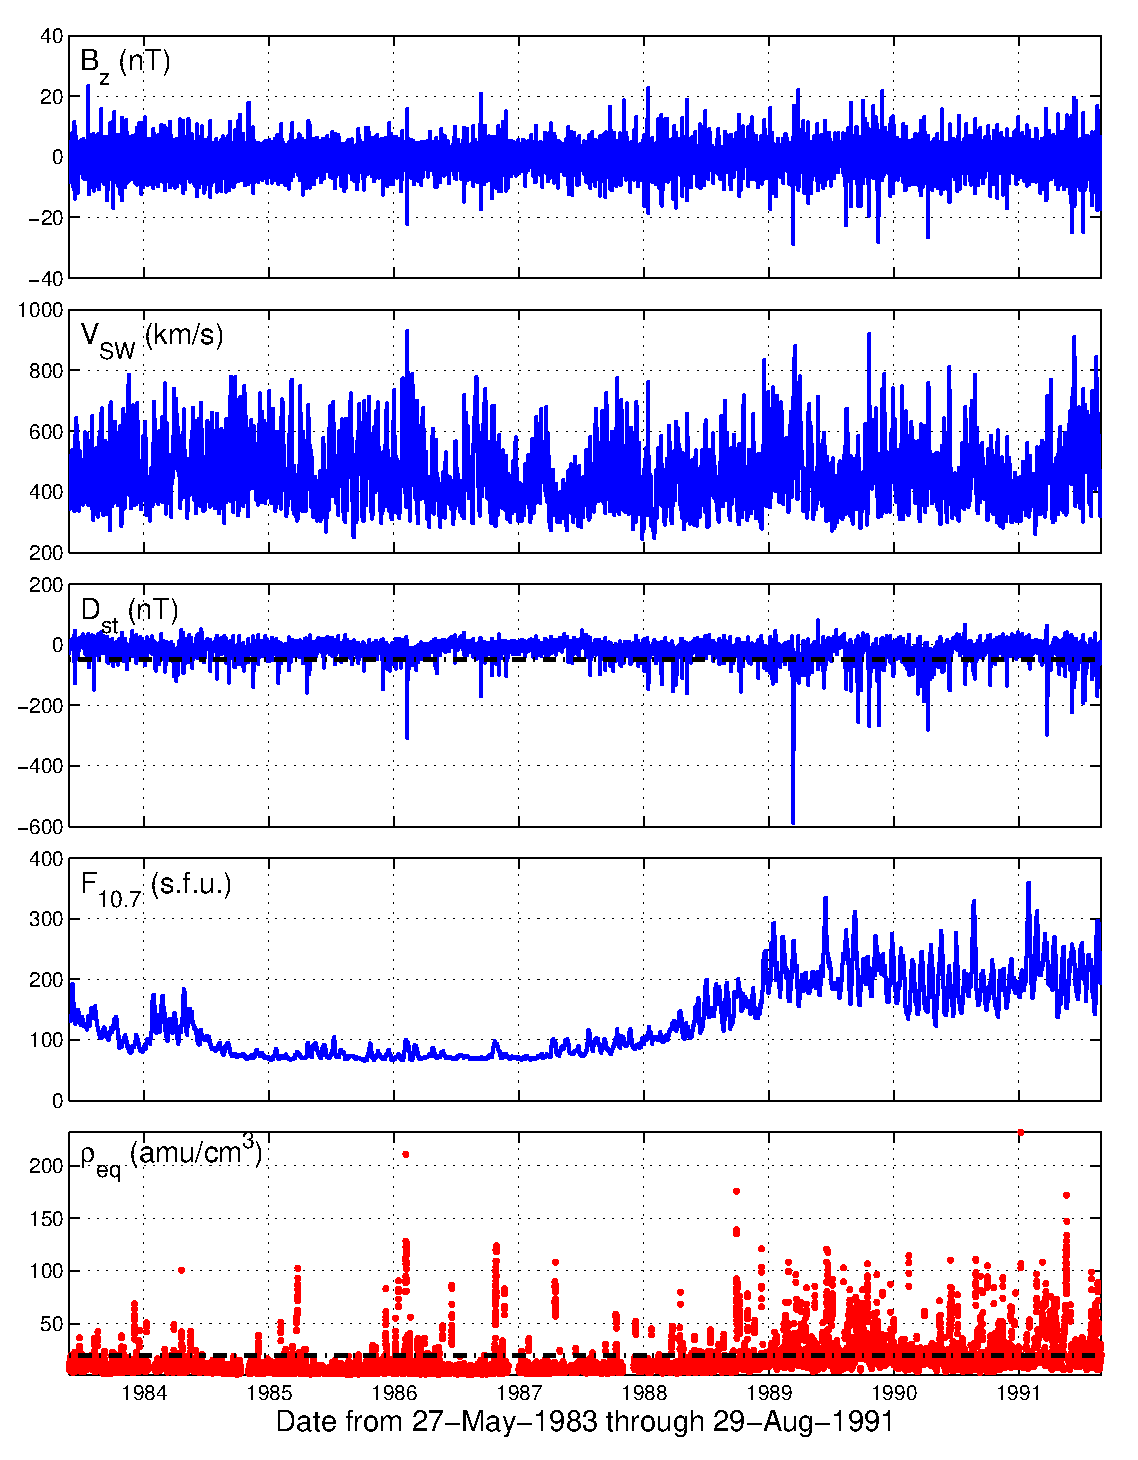
\includegraphics[scale=0.45]{paperfigures/alldata-GOES6-1983-1991.eps}
\caption{Overview of data used in this study. The top four panels show parameters from \cite{Reconstruction} and the bottom panel contains $\rho_{eq}$ based on GOES 6 measurements from \cite{Denton} after interpolation and averaging described in the text. Dashed horizontal lines in the $D_{st}$ and $\rho_{eq}$ panels indicate sample event cutoff thresholds of $D_{st} = -50$~nT and $\rho_{eq} = 40$~amu/cm$^3$}.
\label{AllData}
\end{figure}

\begin{figure}[htp!]
\centering
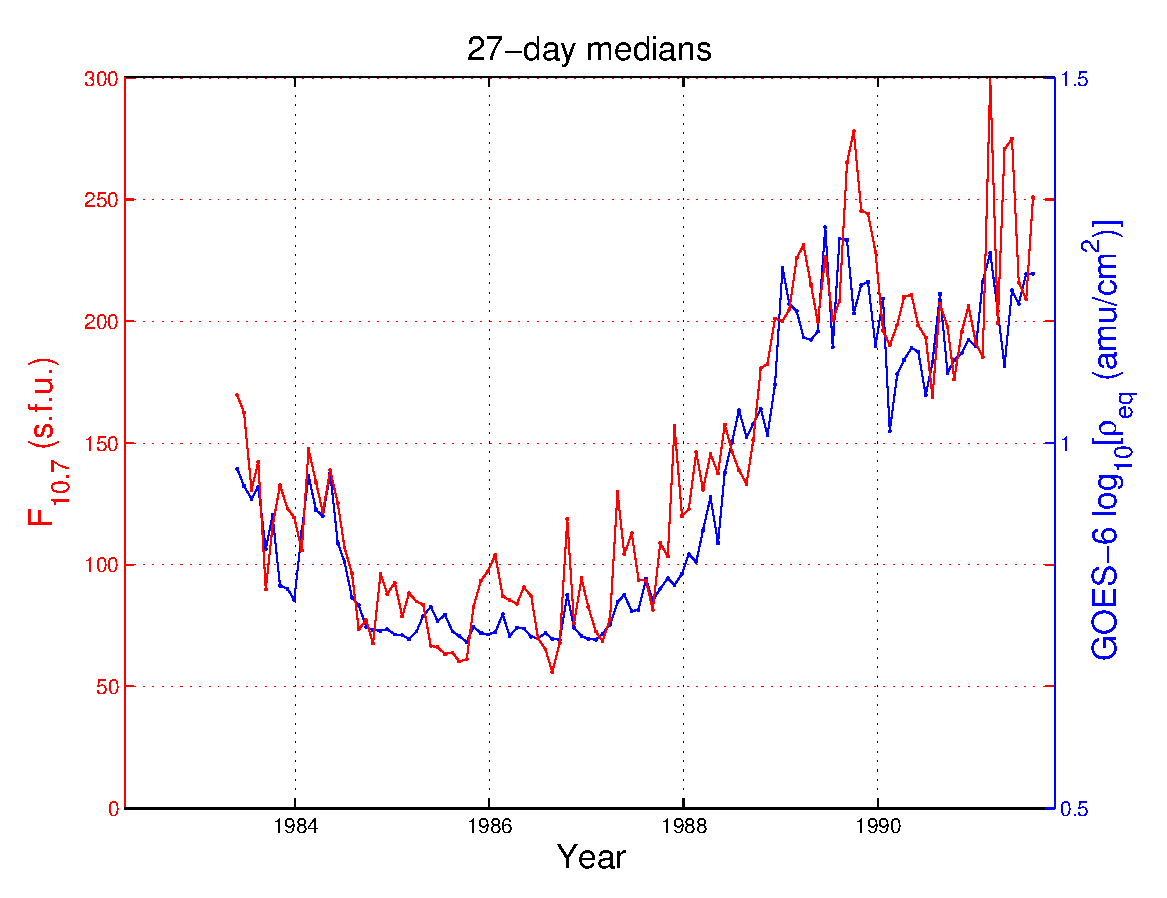
\includegraphics[scale=0.40]{paperfigures/F107MD27d-GOES6.eps}
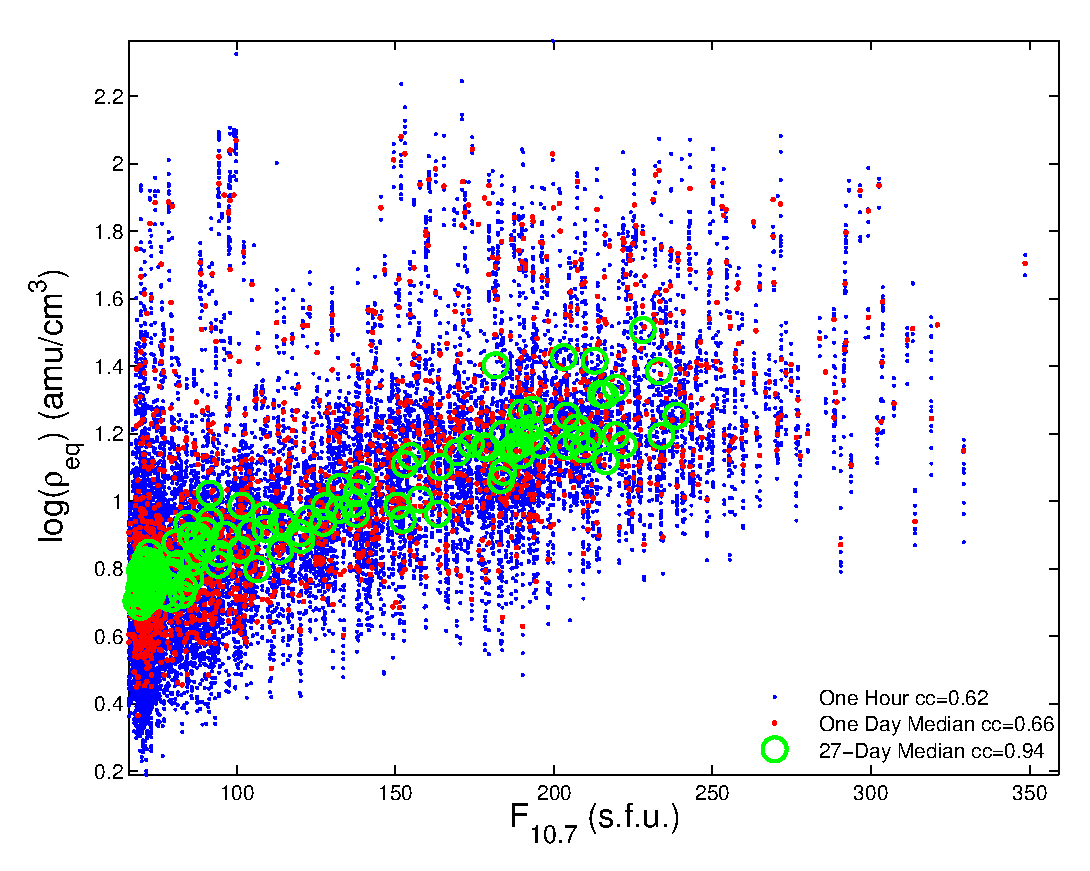
\includegraphics[scale=0.40]{paperfigures/ccplot.eps}
\caption{(a) 27-day averages of $F_{10.7}$ and $\rho_{eq}$. (b) Correlation between $\log(\rho_{eq})$ and $F_{10.7}$ using hour, day, and 27-day averaging intervals; compare to \cite{Takahashi2010} Fig.~14.}
\label{ccplot}
\end{figure}
\clearpage

\begin{figure}[tp!]
\centering
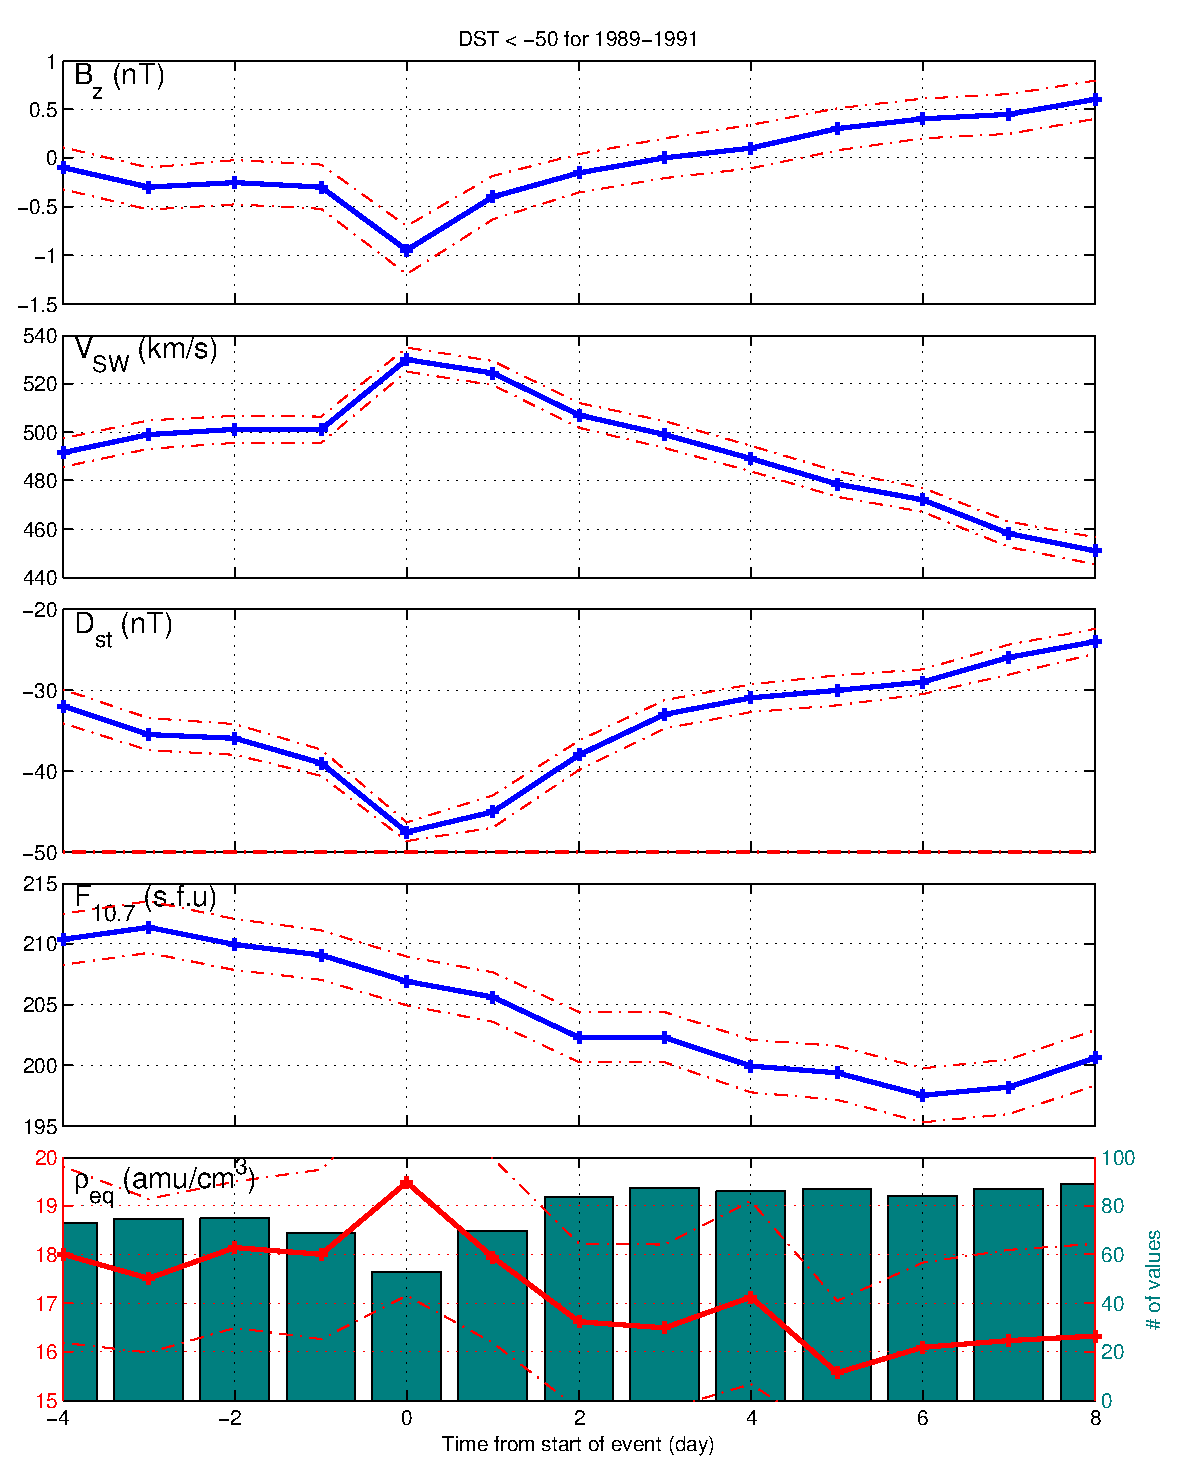
\includegraphics[scale=0.40]{paperfigures/stormavs-dst-50-tak.eps}
\rule[1ex]{5cm}{1pt}
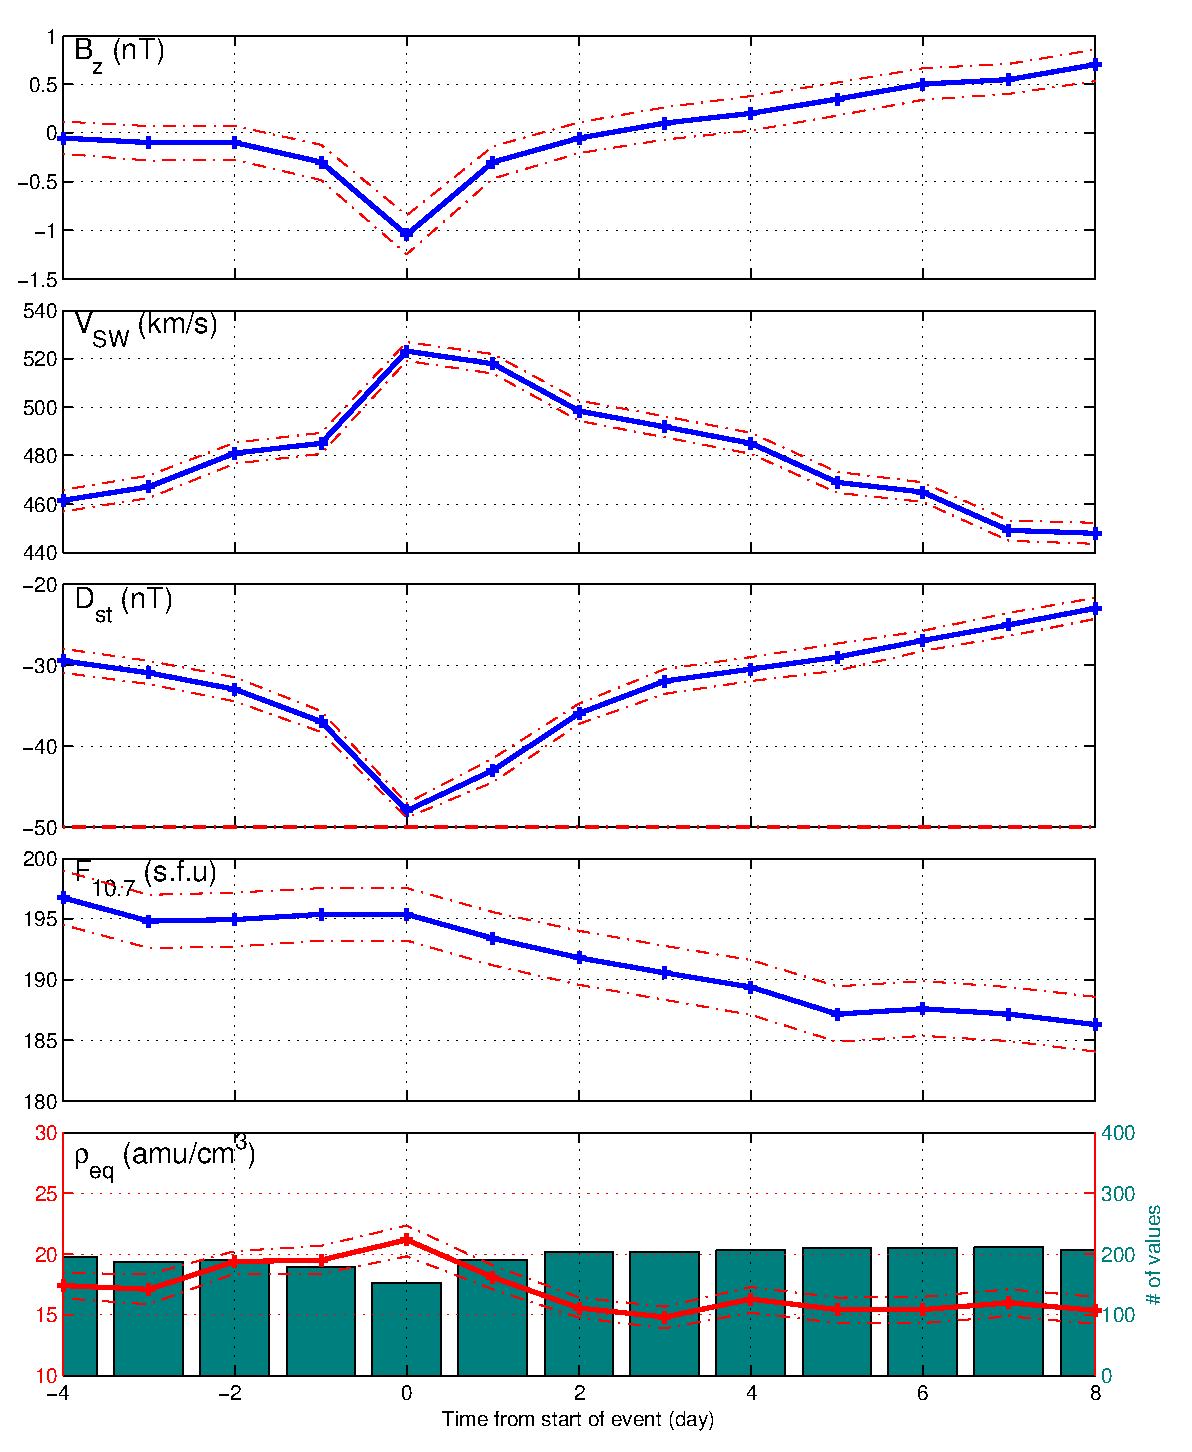
\includegraphics[scale=0.40]{paperfigures/stormavs-dst-day.eps}
\caption{Events in the interval 1989-1991. Upper panel: $D_{st}$ events. Lower panel: Events in the interval 1983-1991.}
\label{DailyAverages}
\end{figure}

\begin{figure}[tp!]
\centering
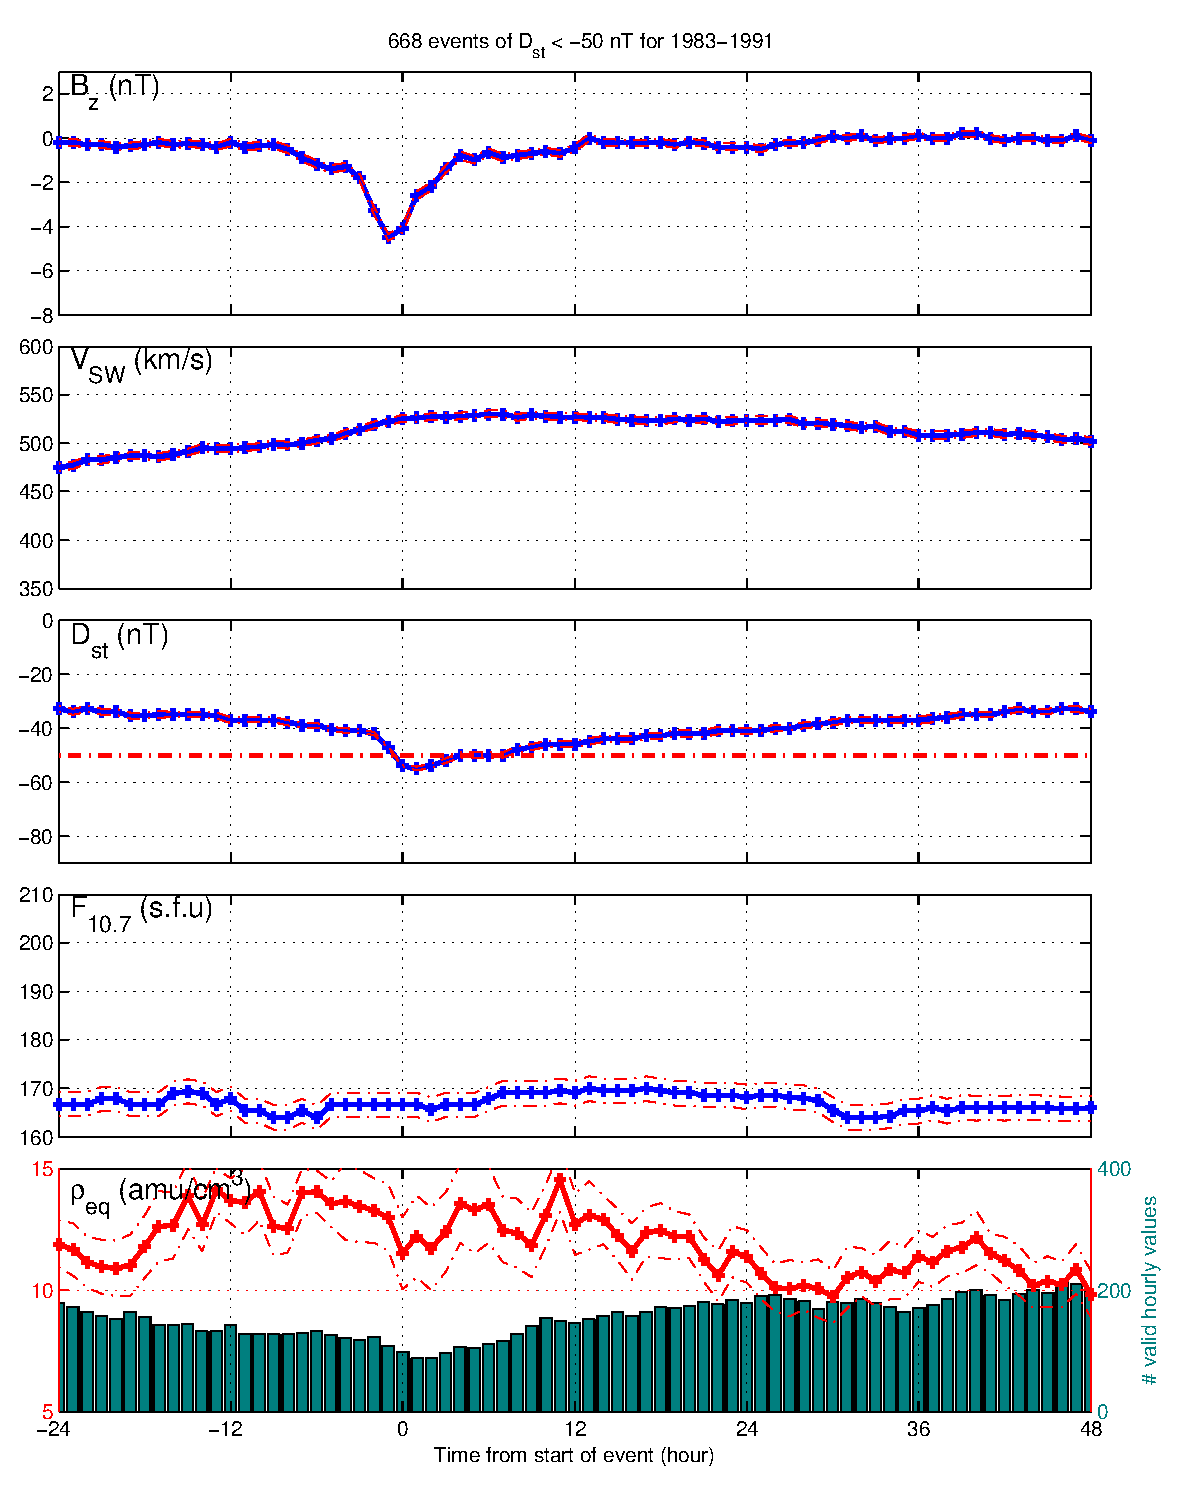
\includegraphics[scale=0.40]{paperfigures/stormavs-dst.eps}
\rule[1ex]{5cm}{1pt}
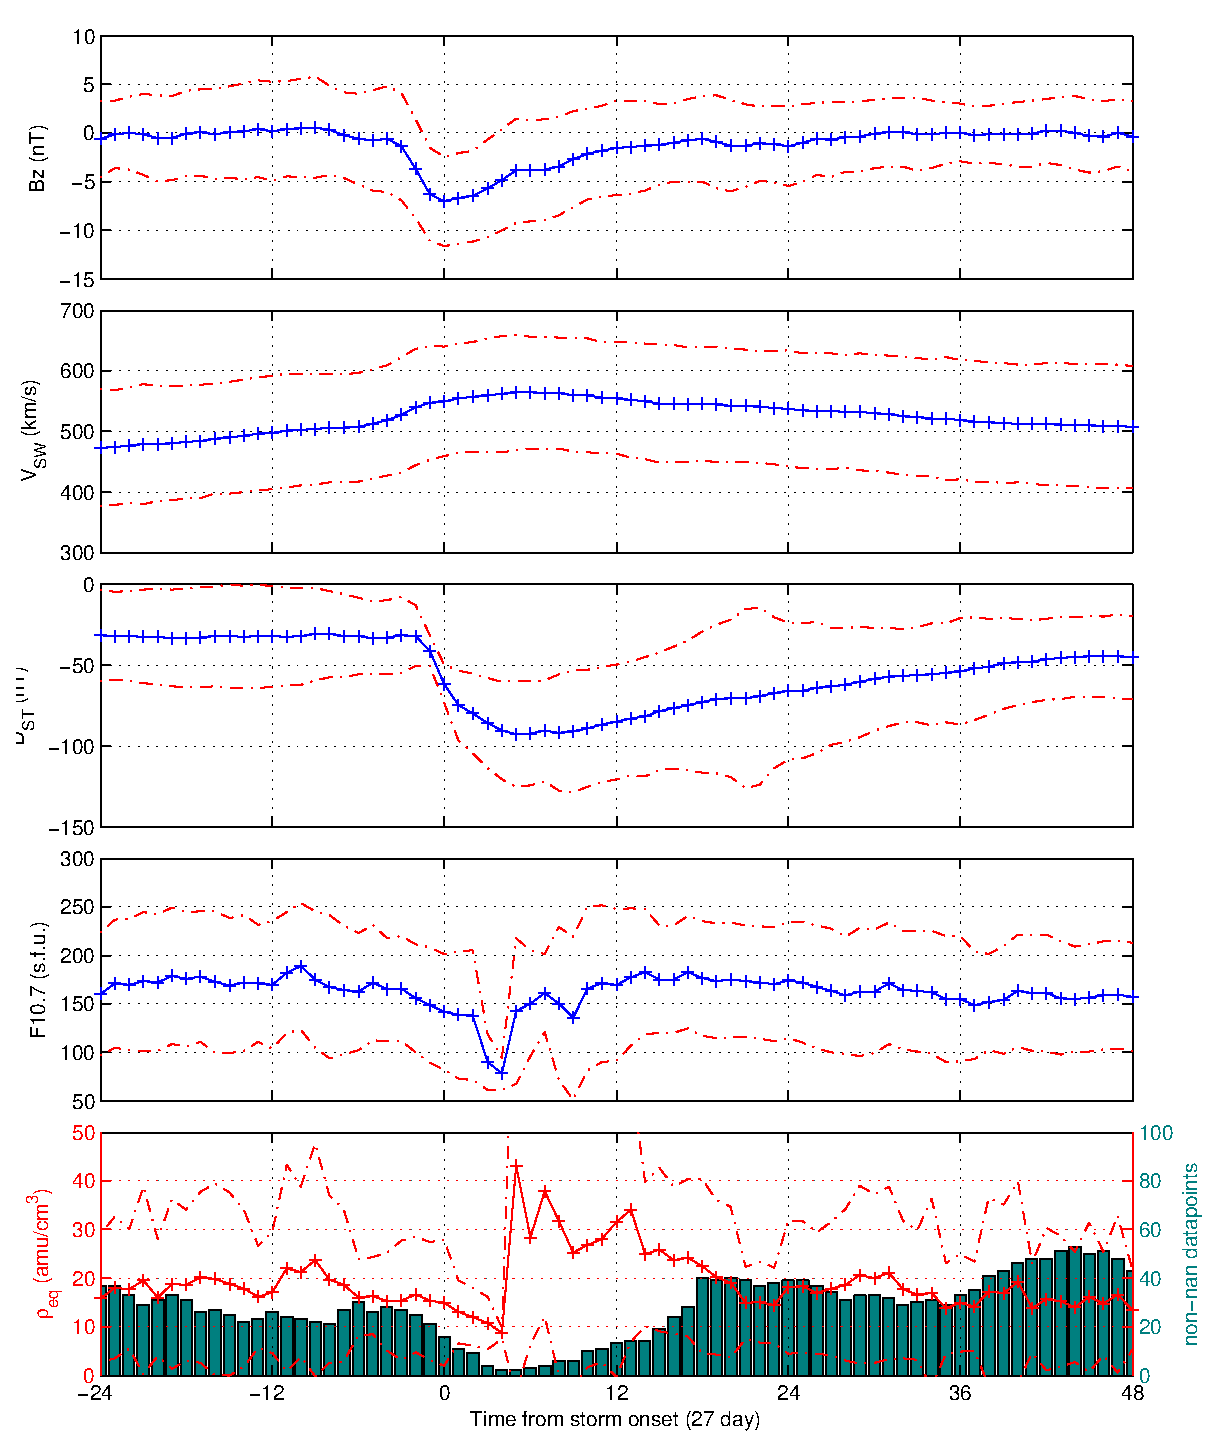
\includegraphics[scale=0.40]{paperfigures/stormavs-dd12.eps}
\caption{(a) Average of solar wind and near-Earth measurements around the time $D_{st}$ crossed below $-50$~nT onset. (b) Same as (a) except for constraint that $D_{st}$ stayed below $-50$~nT for at least 12~hours.}
\label{Storms}
\end{figure}

\clearpage



\begin{figure}[tp!]
\centering
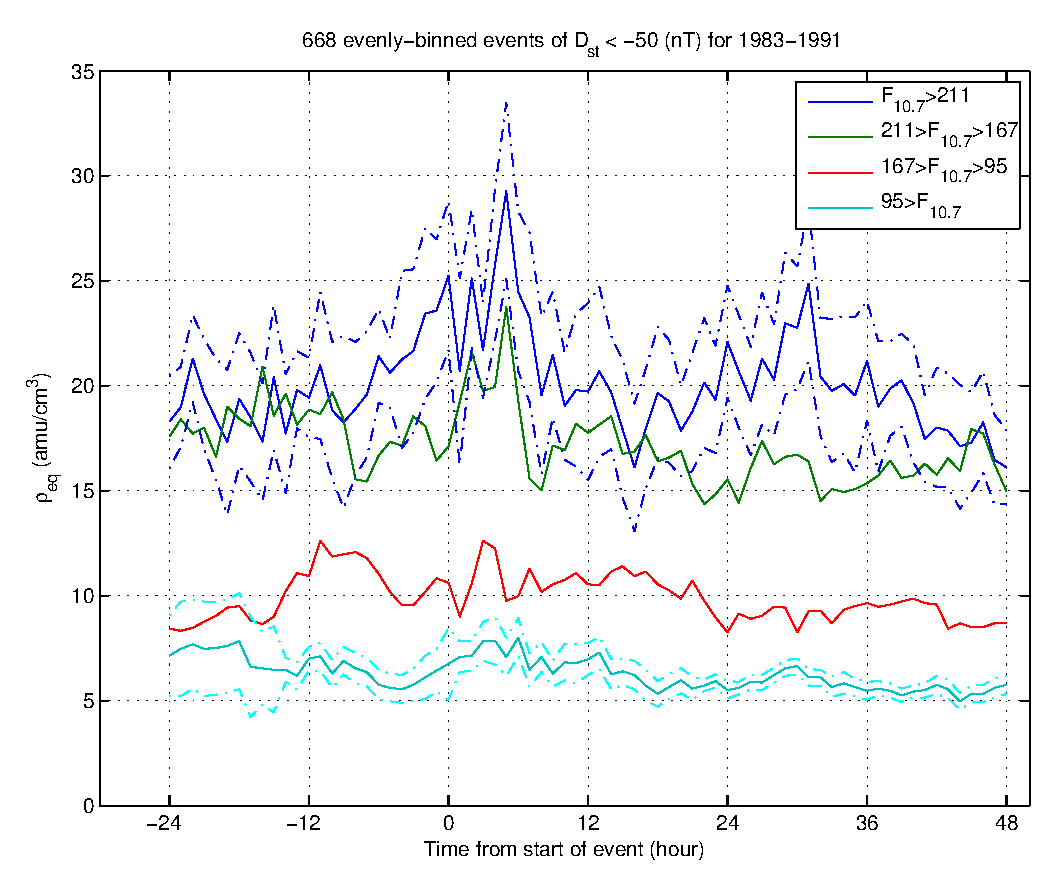
\includegraphics[scale=0.40]{paperfigures/HighLowF107rhoeq.eps}
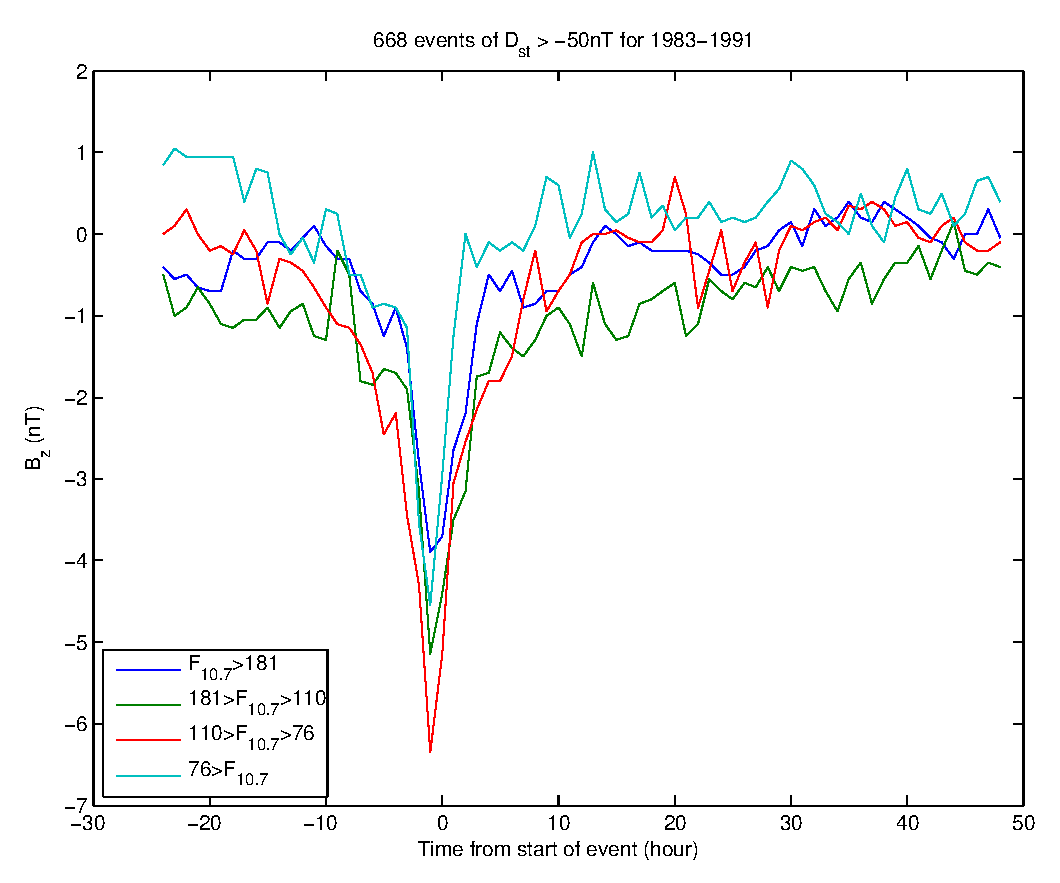
\includegraphics[scale=0.40]{paperfigures/HighLowF107Bz.eps}
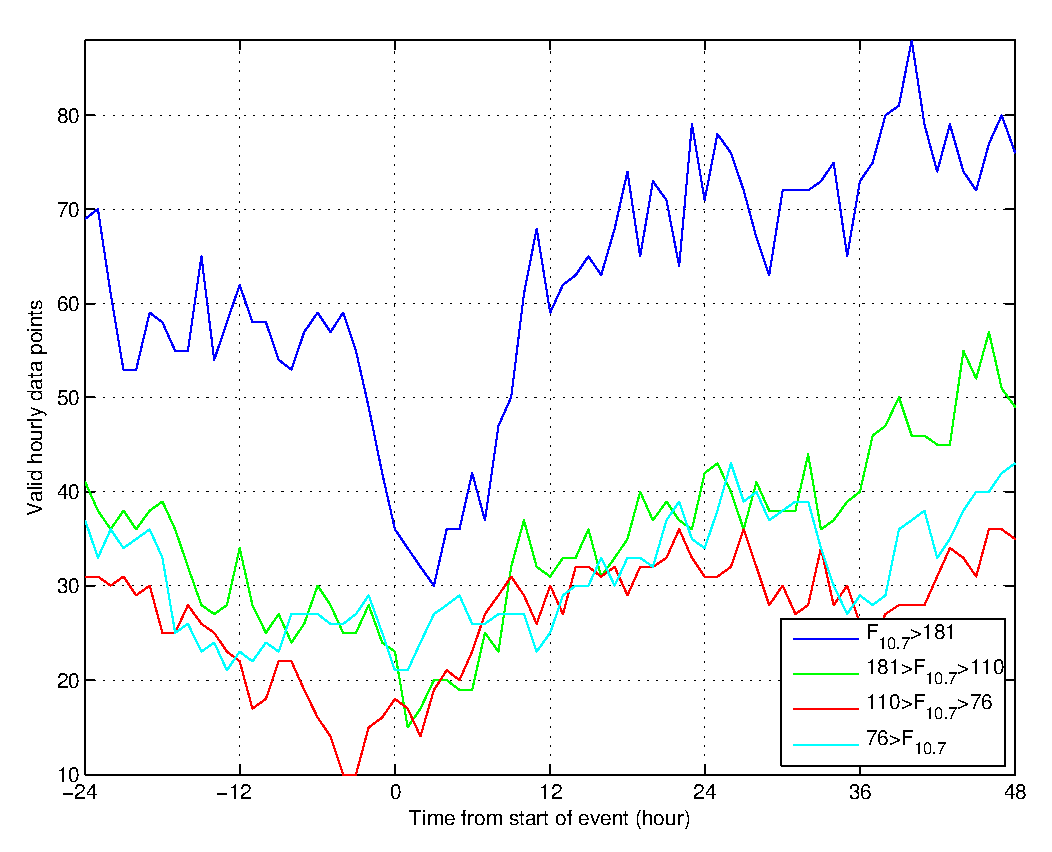
\includegraphics[scale=0.40]{paperfigures/HighLowF107valid.eps}
\caption{Binning events by $F_{10.7}$ value at onset for $\rho_{eq}$ and, in the middle panel, $B_z$. Lower panel shows number of valid points in each bin}
\label{f107bin}
\end{figure}

\clearpage

\section{Appendix}
\hfill

\begin{figure}[htp!]
\centering
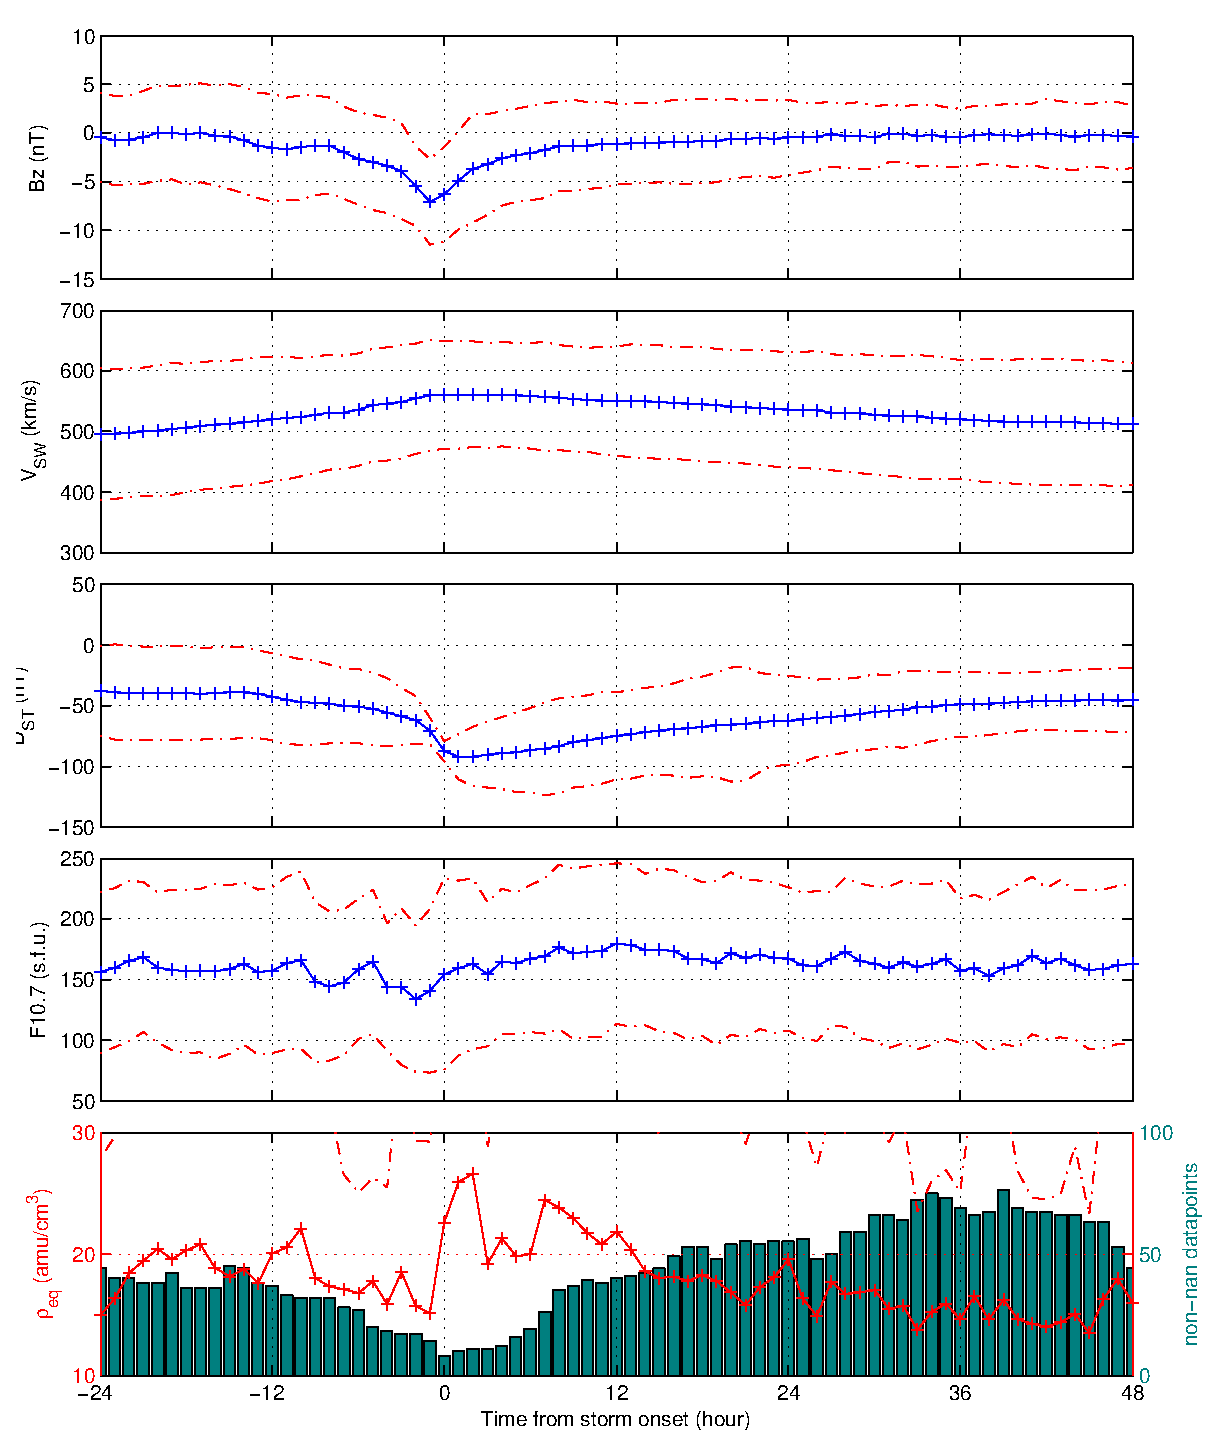
\includegraphics[scale=0.40]{paperfigures/stormavs-d80.eps}
\rule[1ex]{5cm}{1pt}
\caption{(a) Same as Figure \ref{Storms}(a) except with constraint that $D_{st}$ crossed below $-80$~nT }
\label{Dspec}
\end{figure}

\clearpage

\begin{figure}[htp!]
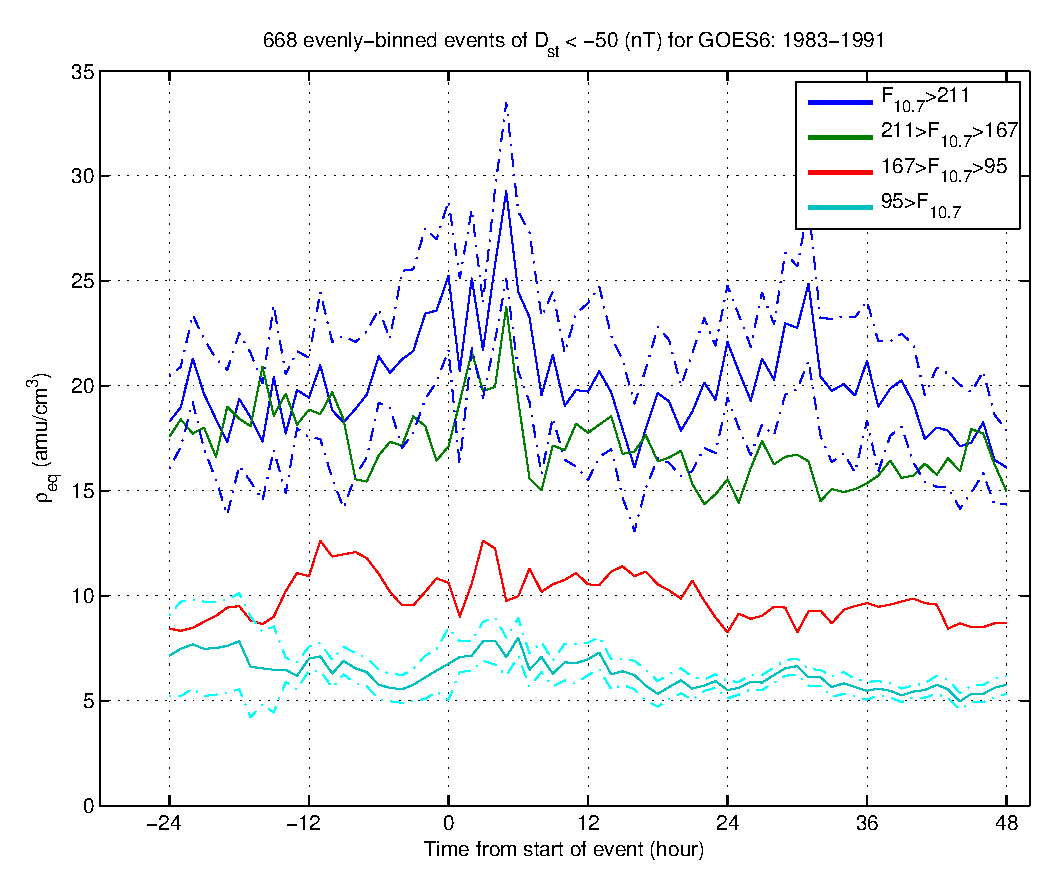
\includegraphics[scale=0.45]{paperfigures/HighLowF107rhoeq-Dst50-GOES6-1983-1991.eps}
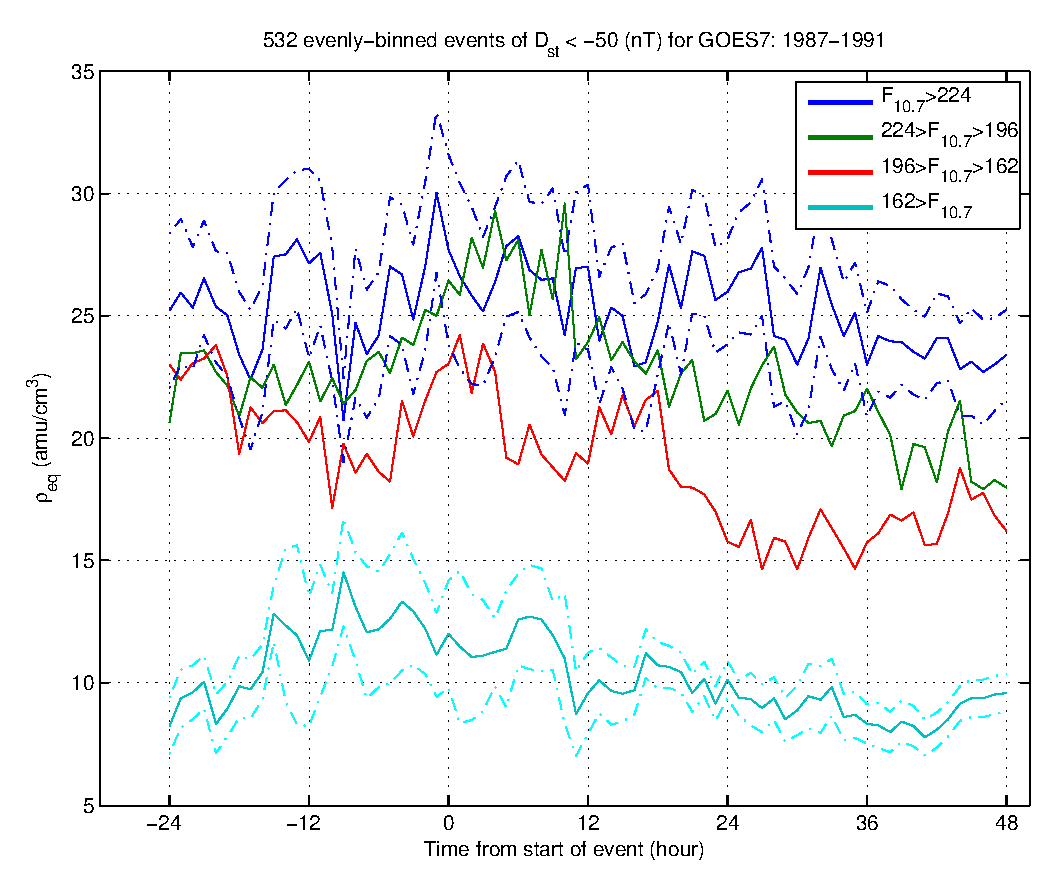
\includegraphics[scale=0.45]{paperfigures/HighLowF107rhoeq-Dst50-GOES7-1987-1991.eps}
\caption{GOES Satellite 6 and 7}
\label{GOES67}
\end{figure}

\begin{figure}[htp!]
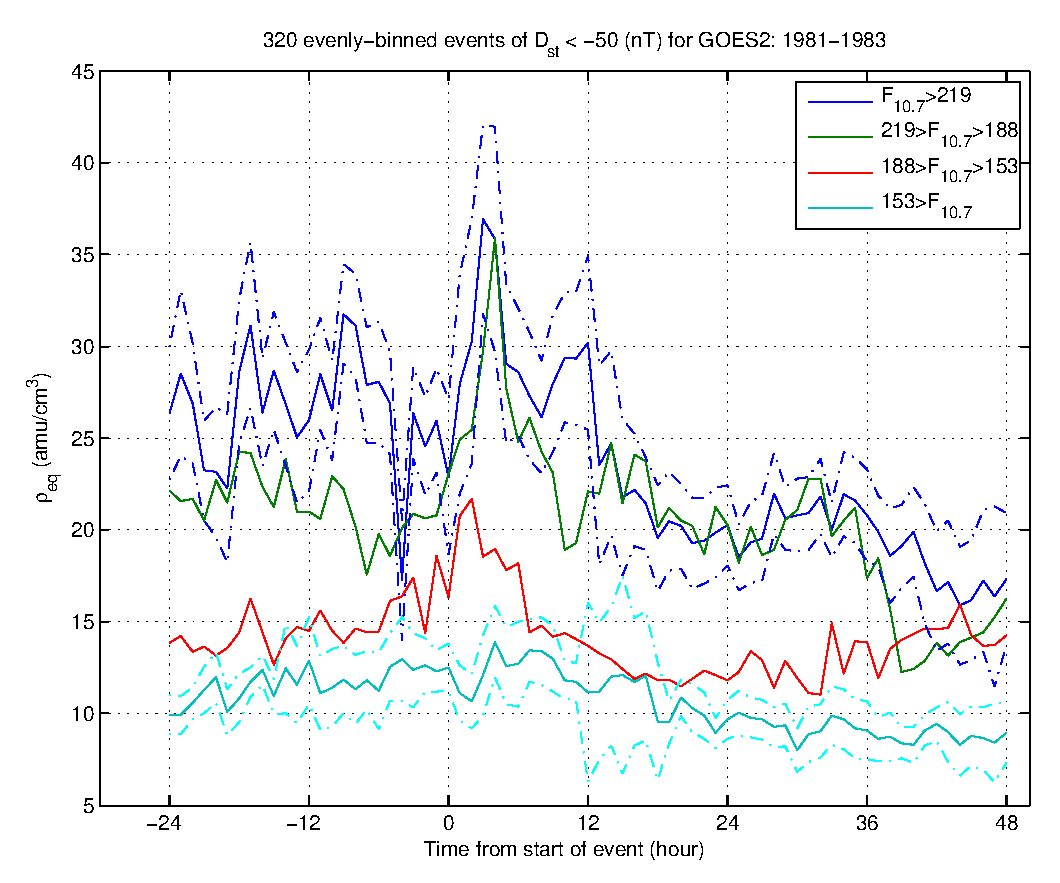
\includegraphics[scale=0.45]{paperfigures/HighLowF107rhoeq-Dst50-GOES2-1981-1983.eps}
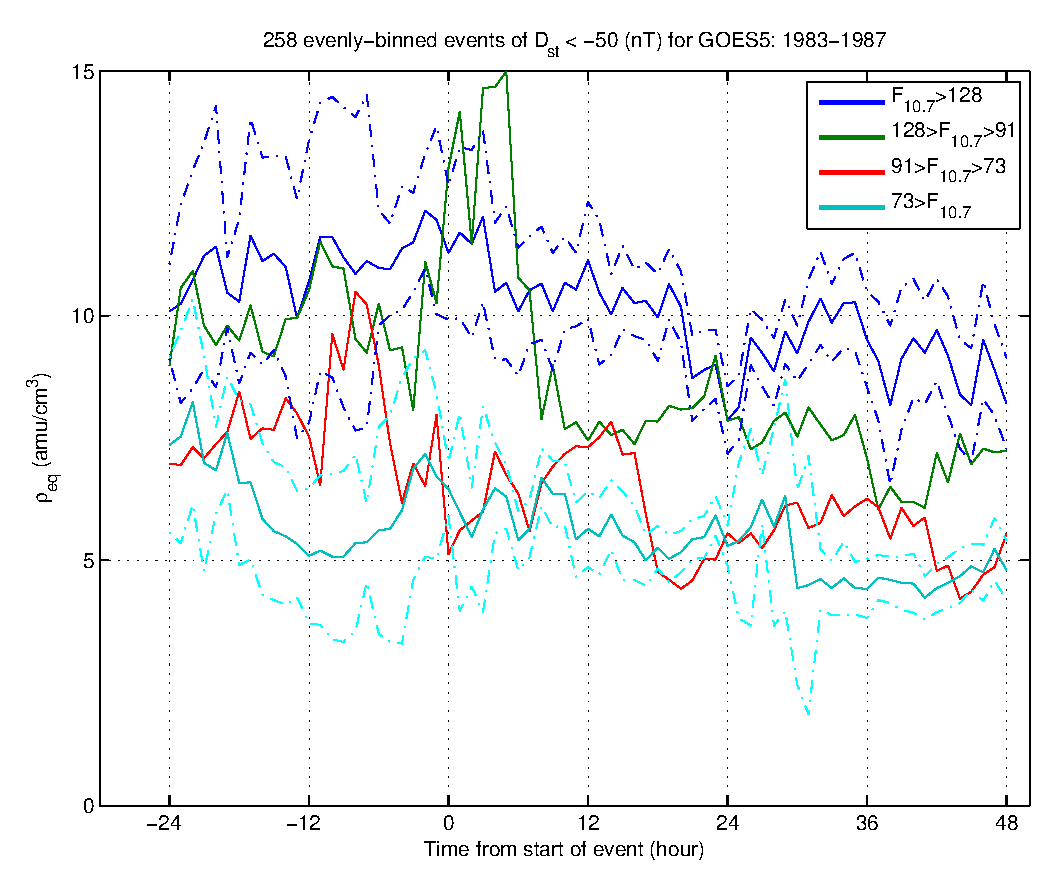
\includegraphics[scale=0.45]{paperfigures/HighLowF107rhoeq-Dst50-GOES5-1983-1987.eps}
\caption{GOES Satellite 2 and 5}
\label{GOES25}
\end{figure}
\clearpage



\begin{figure}[htp!]
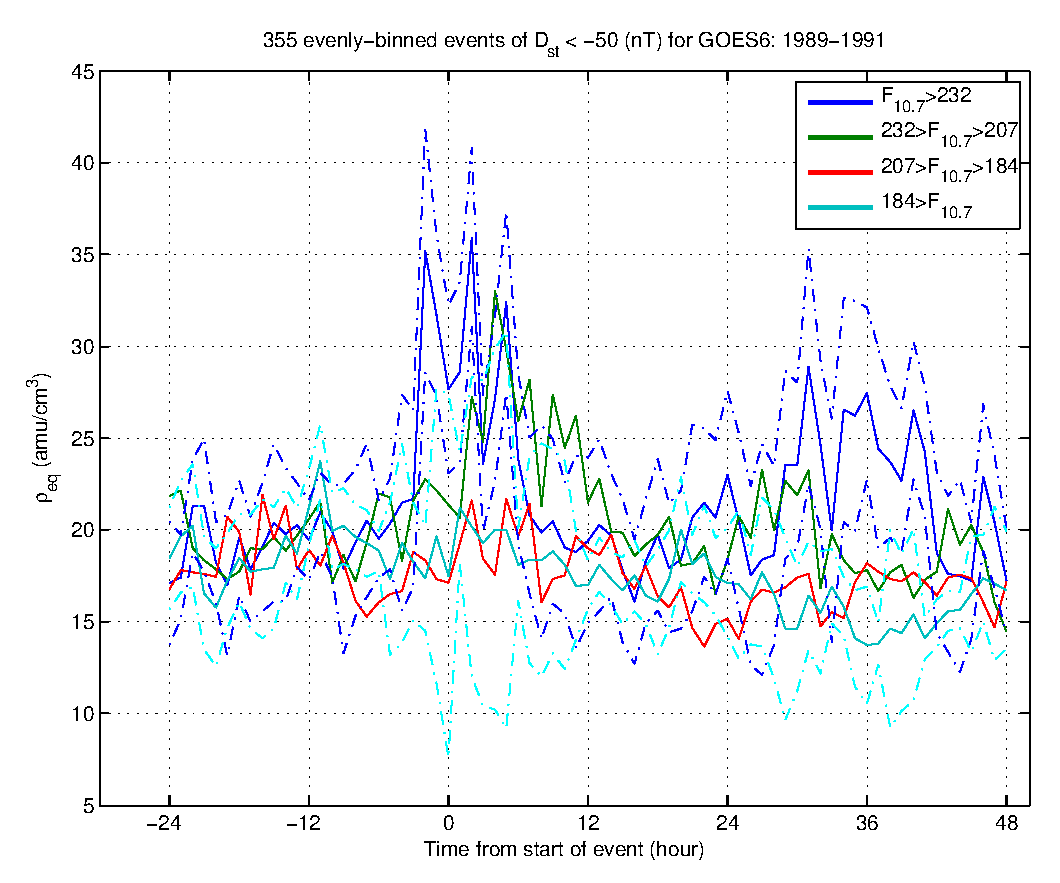
\includegraphics[scale=0.45]{paperfigures/HighLowF107rhoeq-Dst50-GOES6-1989-1991.eps}
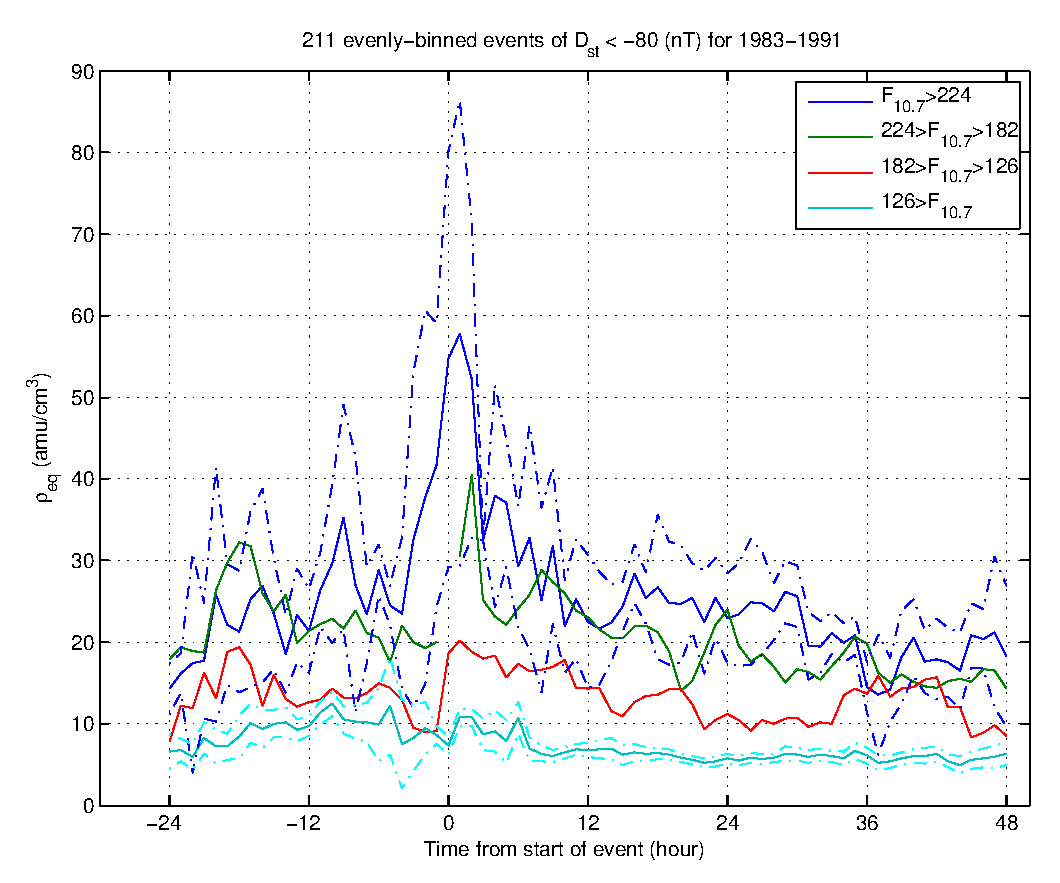
\includegraphics[scale=0.45]{paperfigures/HighLowF107rhoeq-Dst80.eps}
\caption{Top: GOES 6 from 89-91 (compare to Takahashi 2010). Bottom:  $D_{st}<-80$~nT.}
\end{figure}


\begin{figure}[htp!]
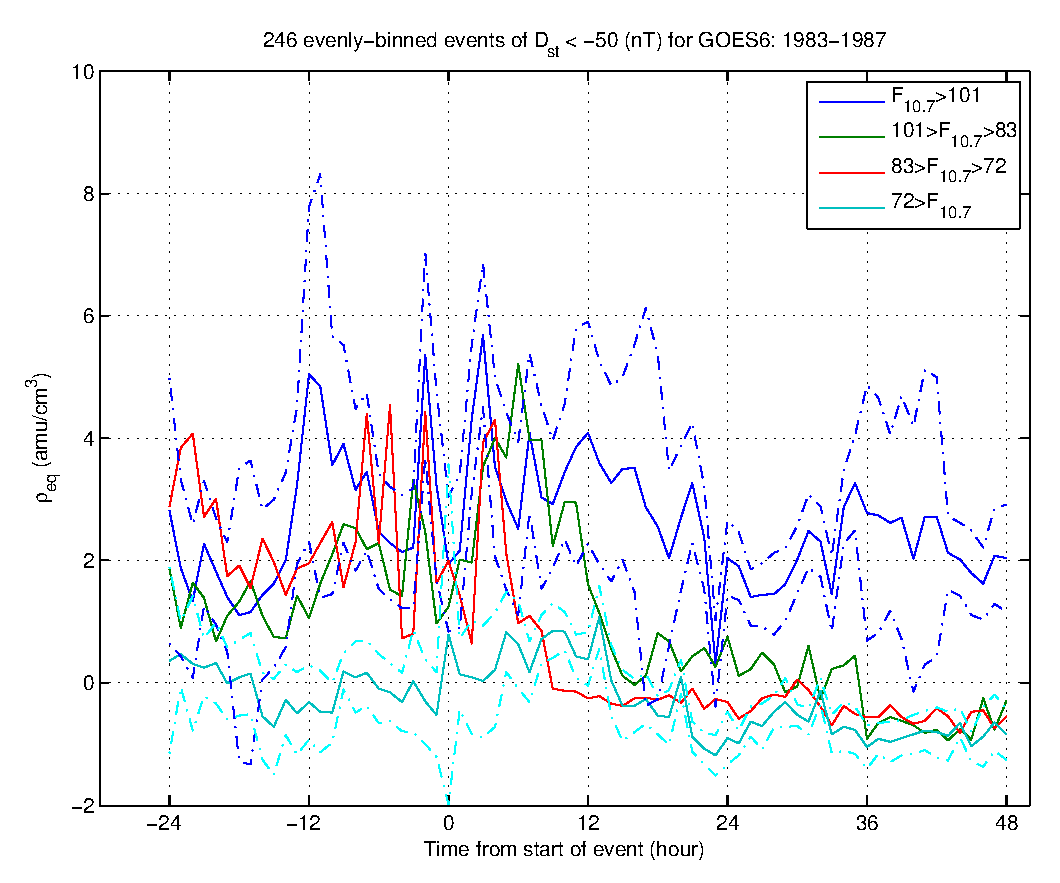
\includegraphics[scale=0.45]{paperfigures/HighLowF107rhoeq-Dst50-GOES6-1983-1987.eps}
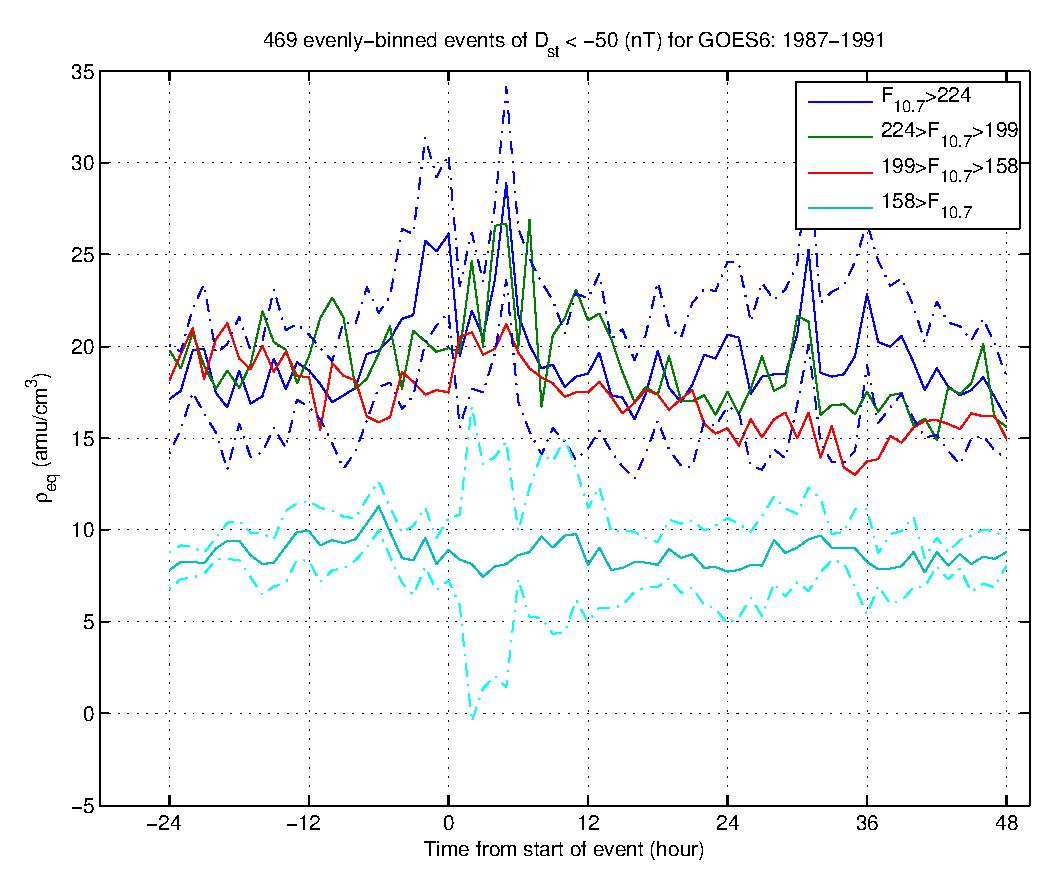
\includegraphics[scale=0.45]{paperfigures/HighLowF107rhoeq-Dst50-GOES6-1987-1991.eps}
\caption{GOES 6 from 83-87 and 87-91}
\end{figure}
\clearpage



\hfill
\begin{figure}[htp!]
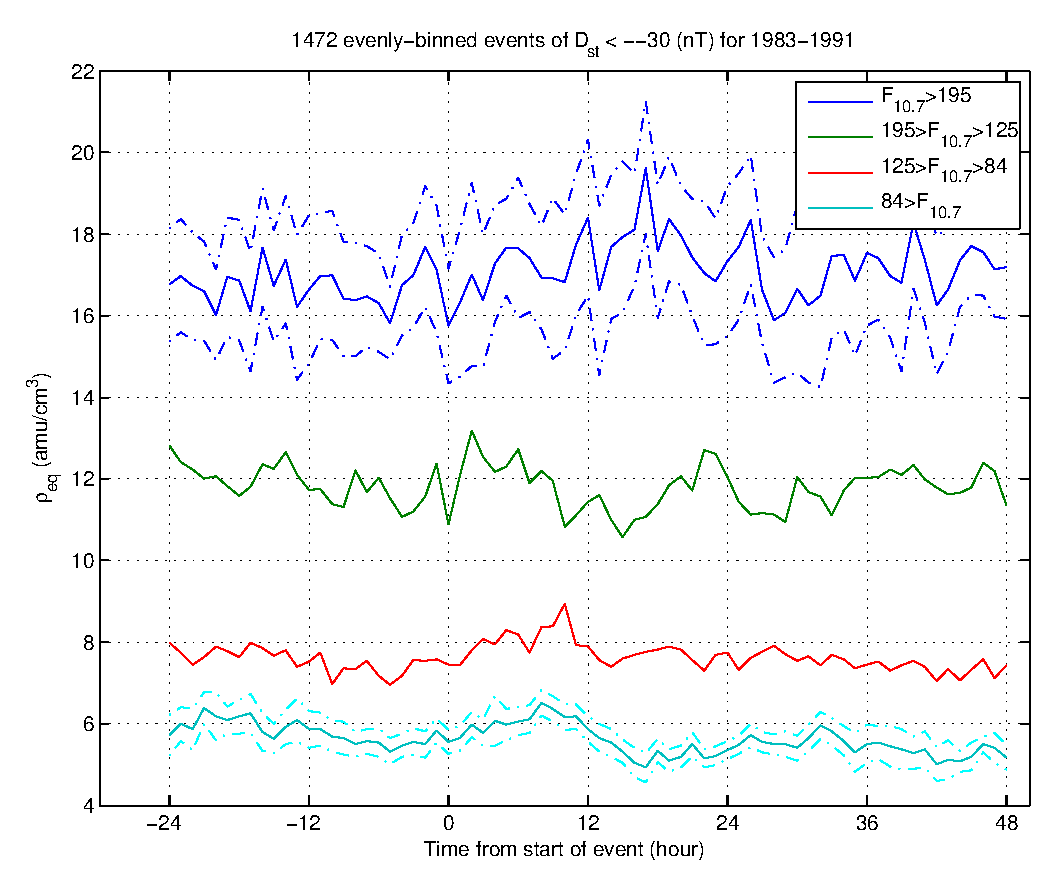
\includegraphics[scale=0.45]{paperfigures/HighLowF107rhoeq-Dst30.eps}
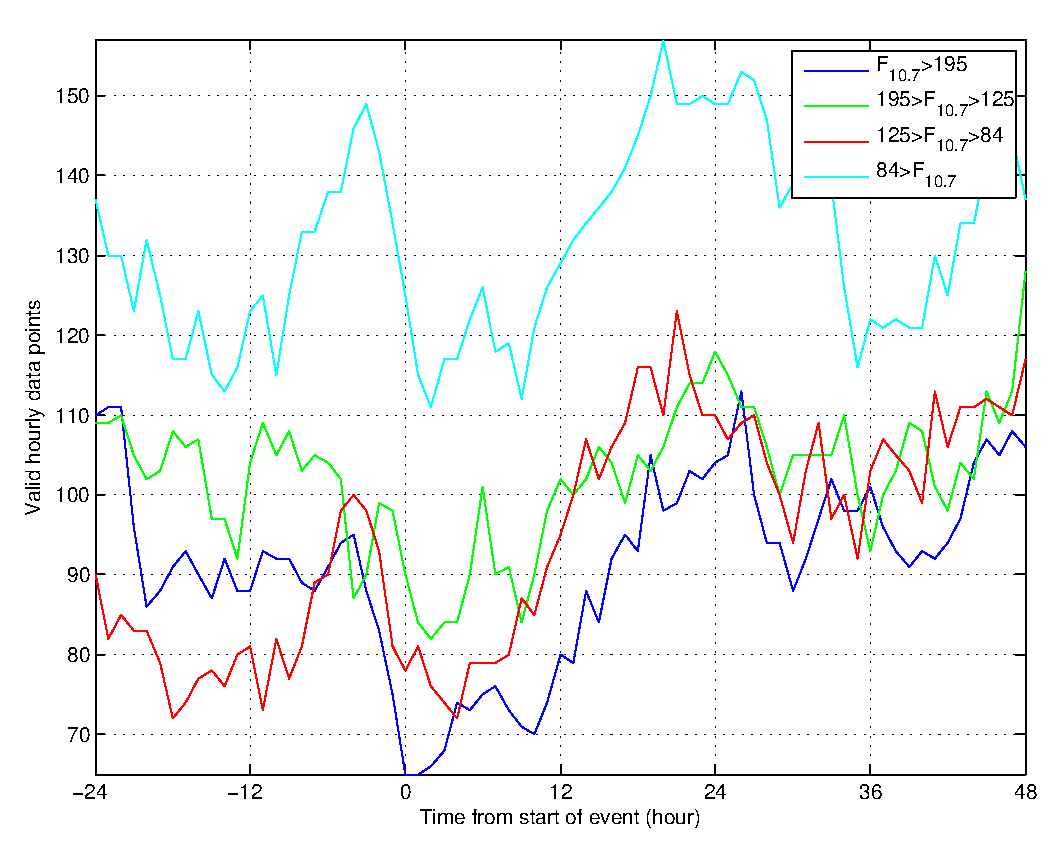
\includegraphics[scale=0.45]{paperfigures/HighLowF107rhoeq-Dst30-valid.eps}
\caption{$D_{st} < -30$ nT events, $\rho_{eq}$ binned by $F_{10.7}$. Lower panel: valid hourly points}
\end{figure}
\hfill
\begin{figure}[htp!]
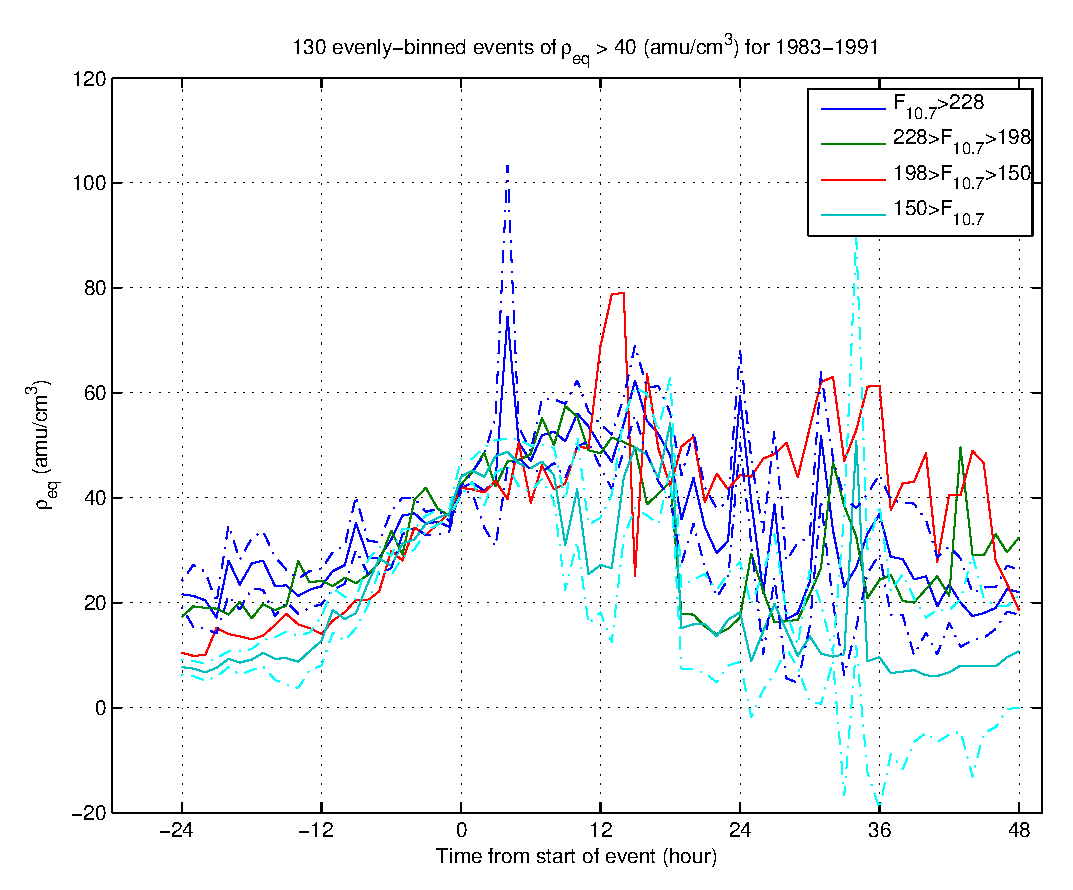
\includegraphics[scale=0.45]{paperfigures/HighLowF107rhoeq-rhoeq40.eps}
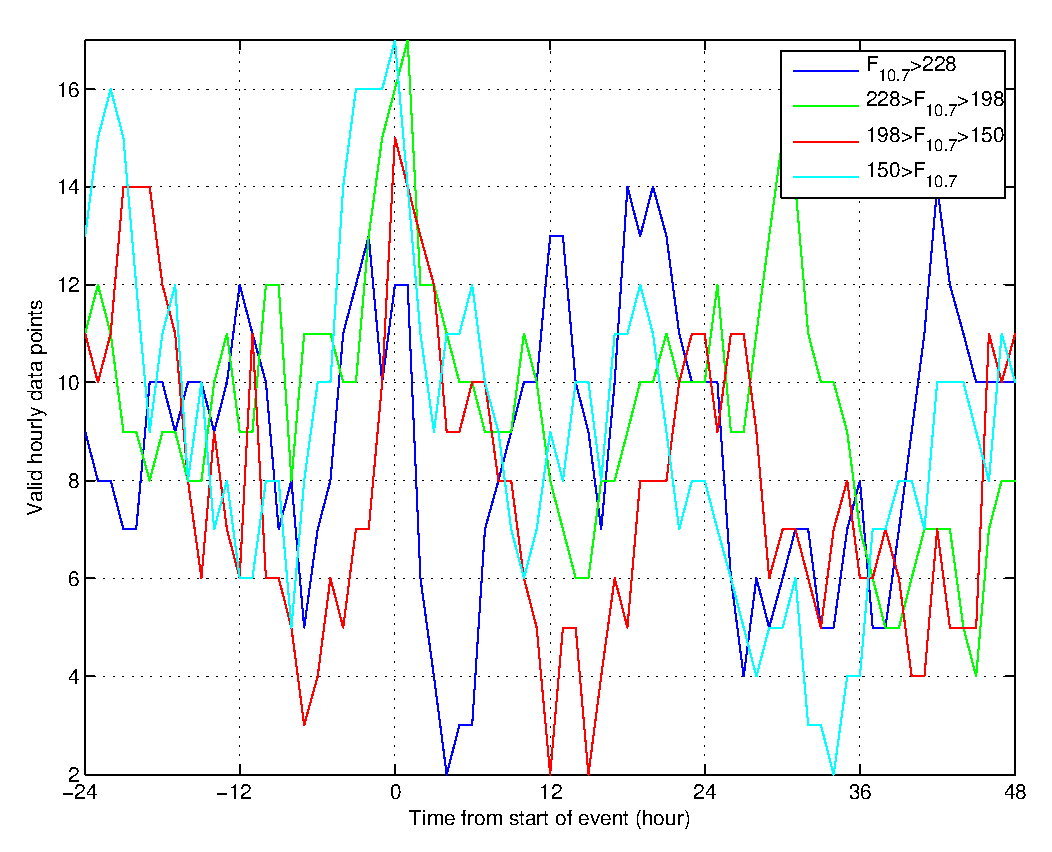
\includegraphics[scale=0.45]{paperfigures/HighLowF107rhoeq-rhoeq40-valid.eps}
\caption{$\rho_{eq} > 40$ amu/cm$^3$ events, $\rho_{eq}$ binned by $F_{10.7}$}
\end{figure}
\clearpage

\begin{figure}[htp!]
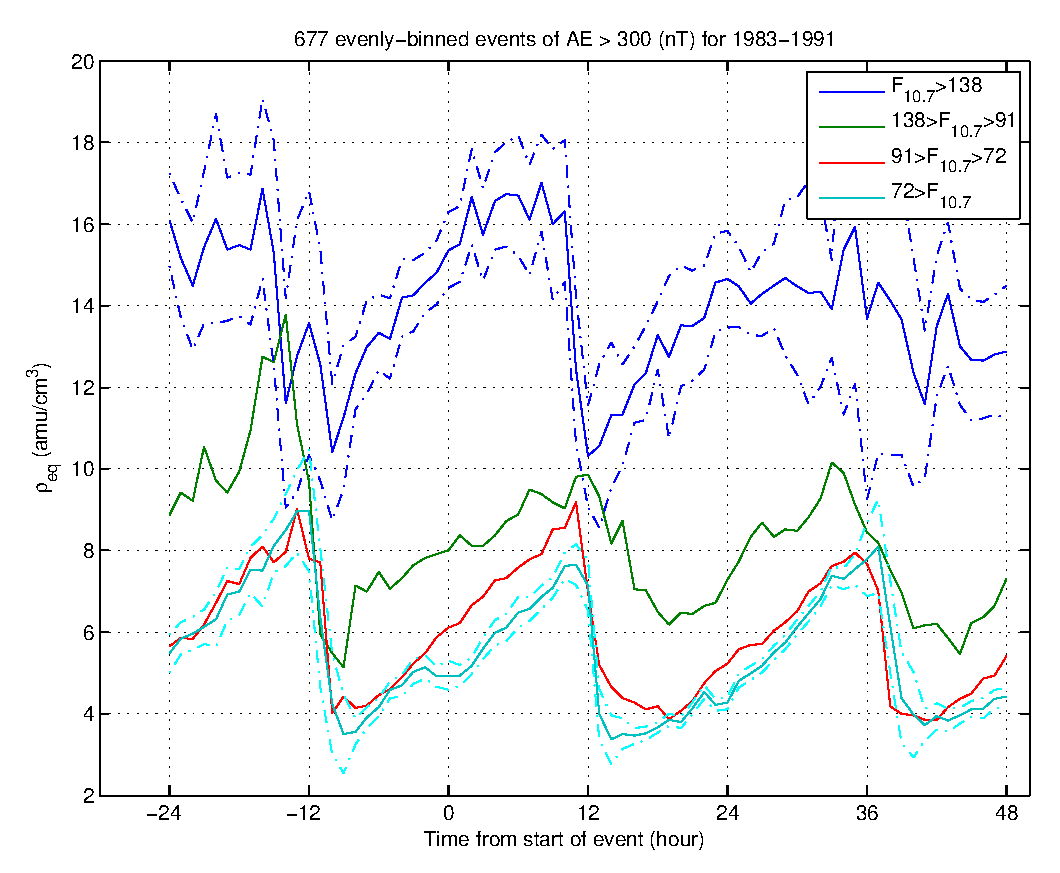
\includegraphics[scale=0.40]{paperfigures/HighLowF107rhoeq-AE300.eps}
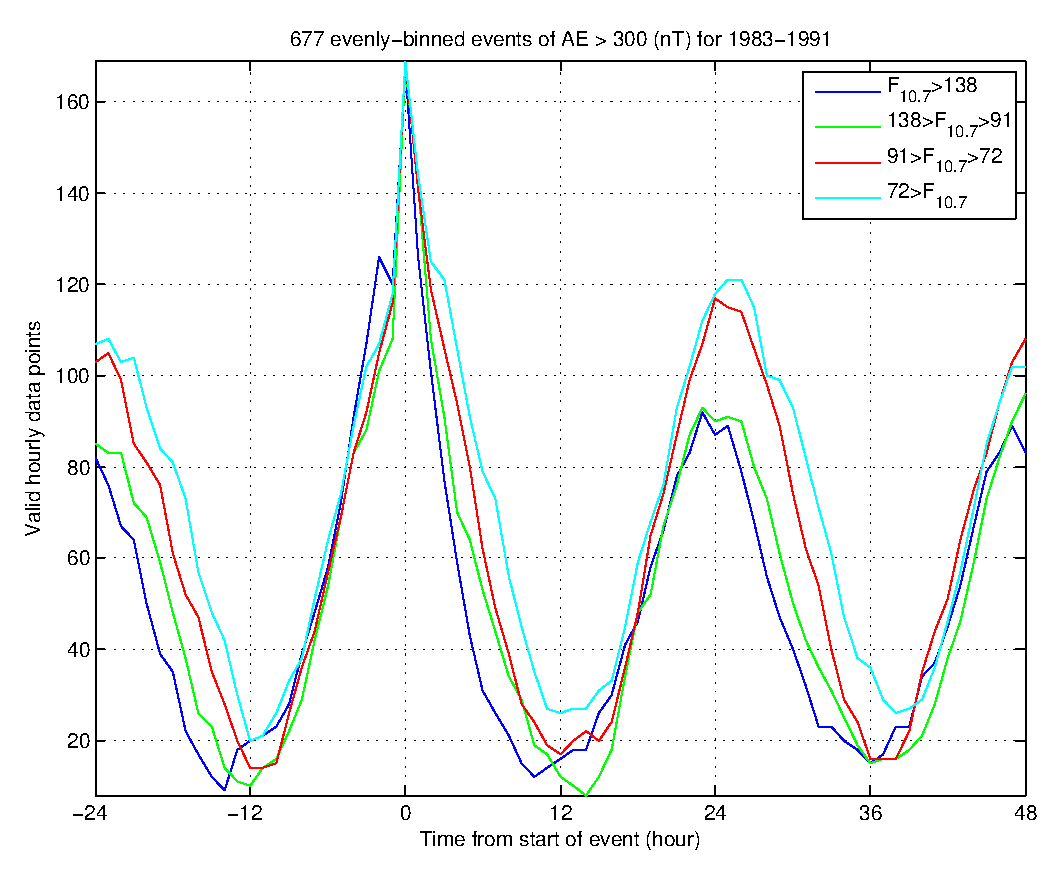
\includegraphics[scale=0.40]{paperfigures/HighLowF107rhoeq-AE300-valid.eps}
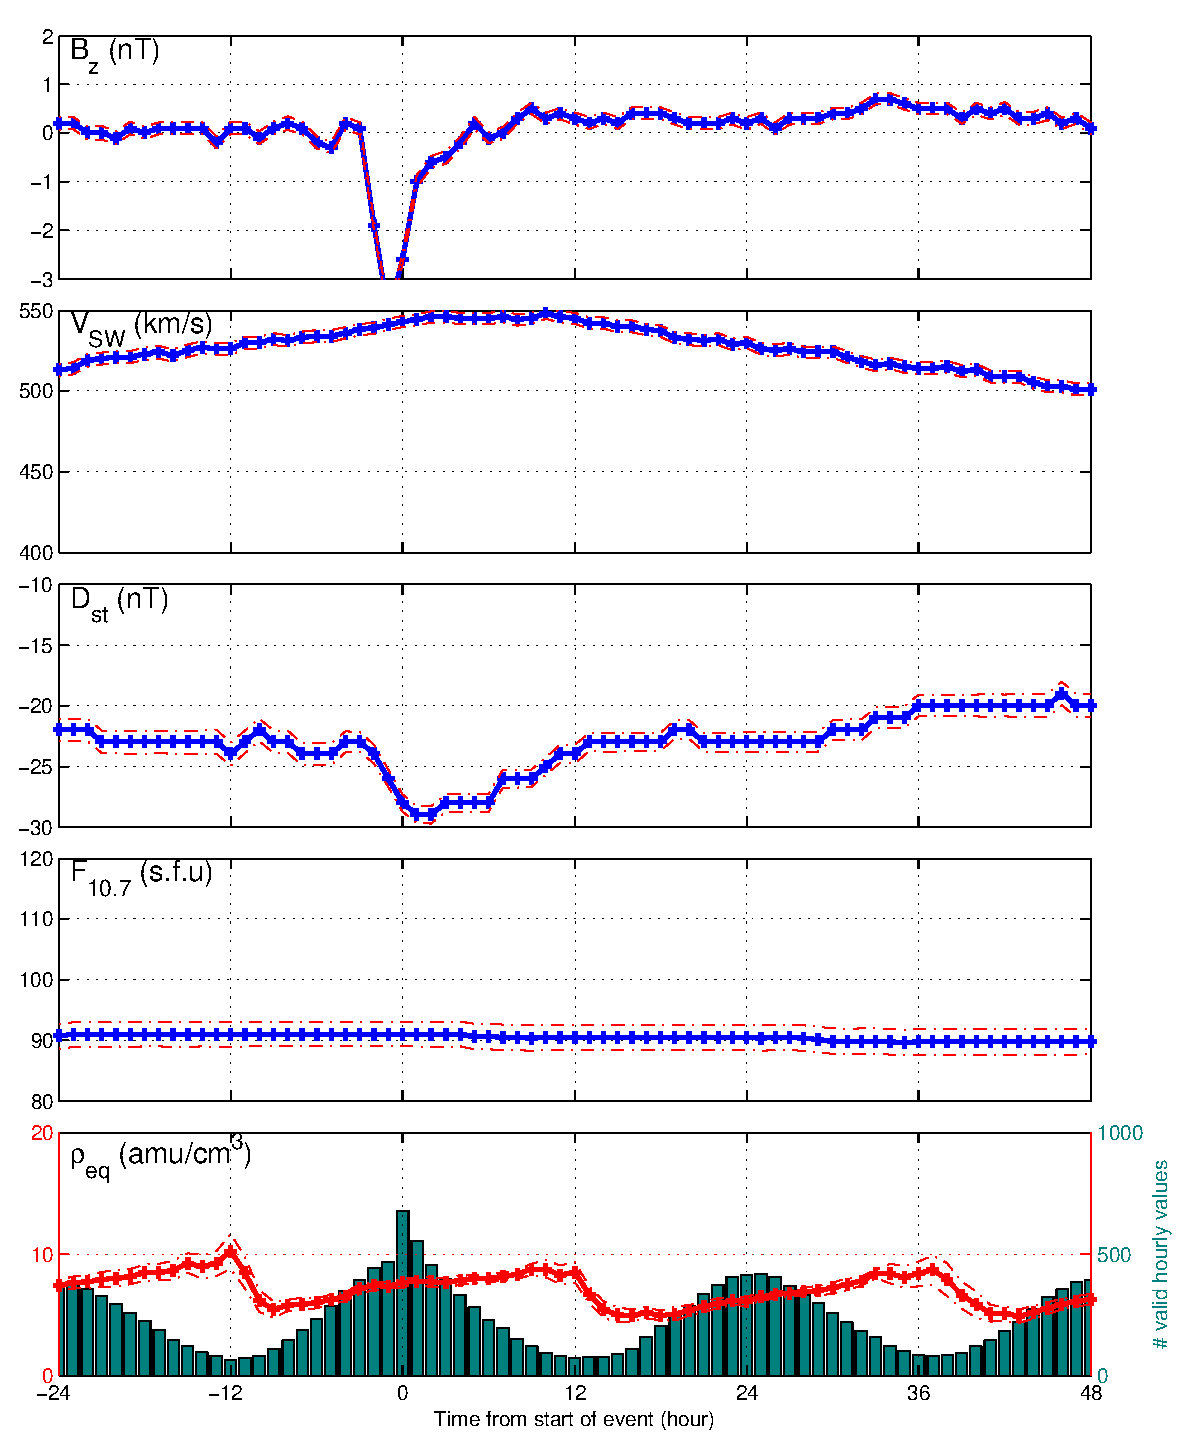
\includegraphics[scale=0.35]{paperfigures/stormavs-AE.eps}
\caption{Top: $AE > 400$ nT events, $\rho_{eq}$ binned by $F_{10.7}$ Bottom: averages of $AE > 400$ events}
\end{figure}
\hfill
\begin{figure}[htp!]
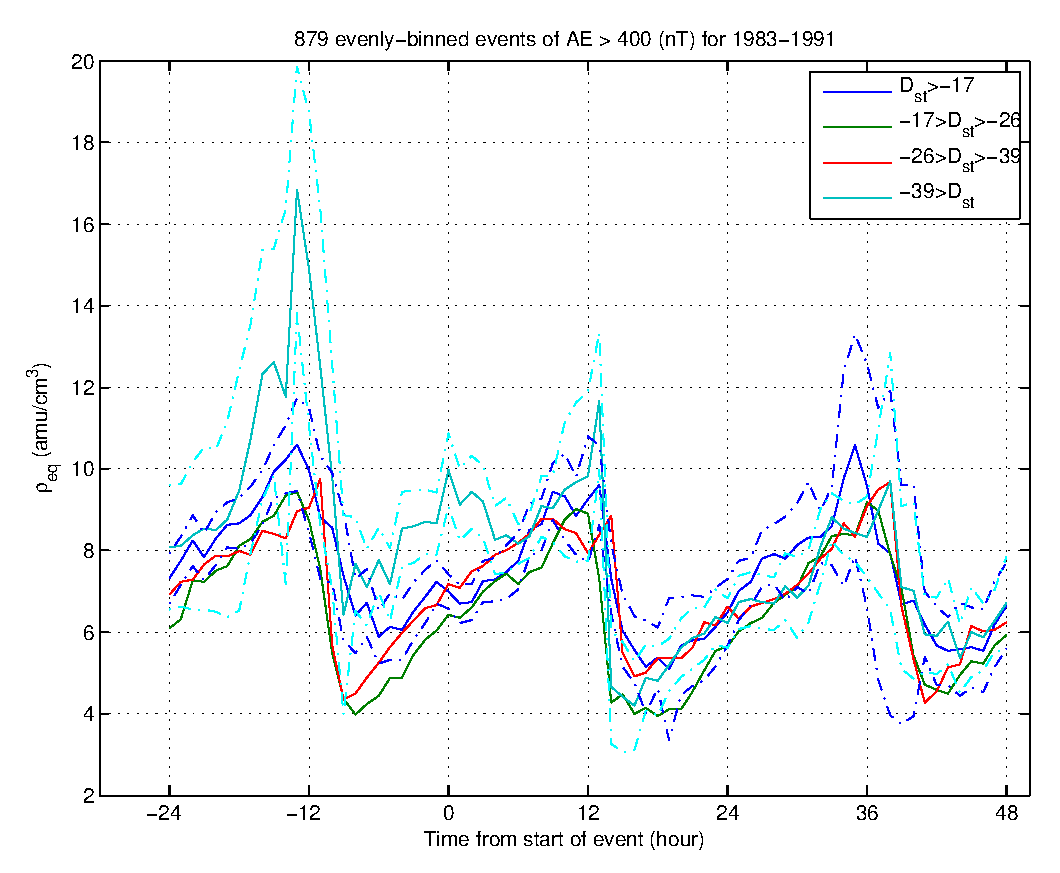
\includegraphics[scale=0.45]{paperfigures/HighLowDstrhoeq-AE400.eps}
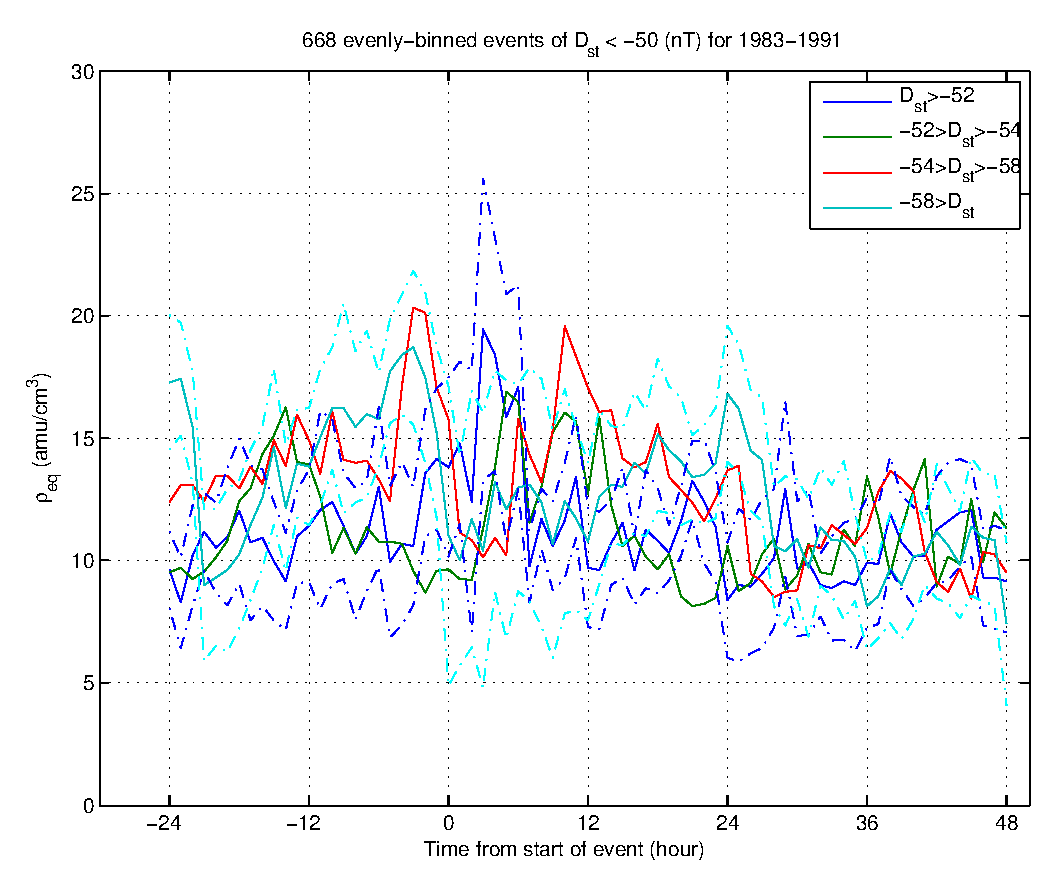
\includegraphics[scale=0.45]{paperfigures/HighLowDstrhoeq-Dst50.eps}
\caption{Top: $AE > 400$ nT events. Bottom: $D_{st} < -50$ nT events. Both $\rho_{eq}$ binned by $D_{st}$.}
\end{figure}
\clearpage

\begin{figure}[htp!]
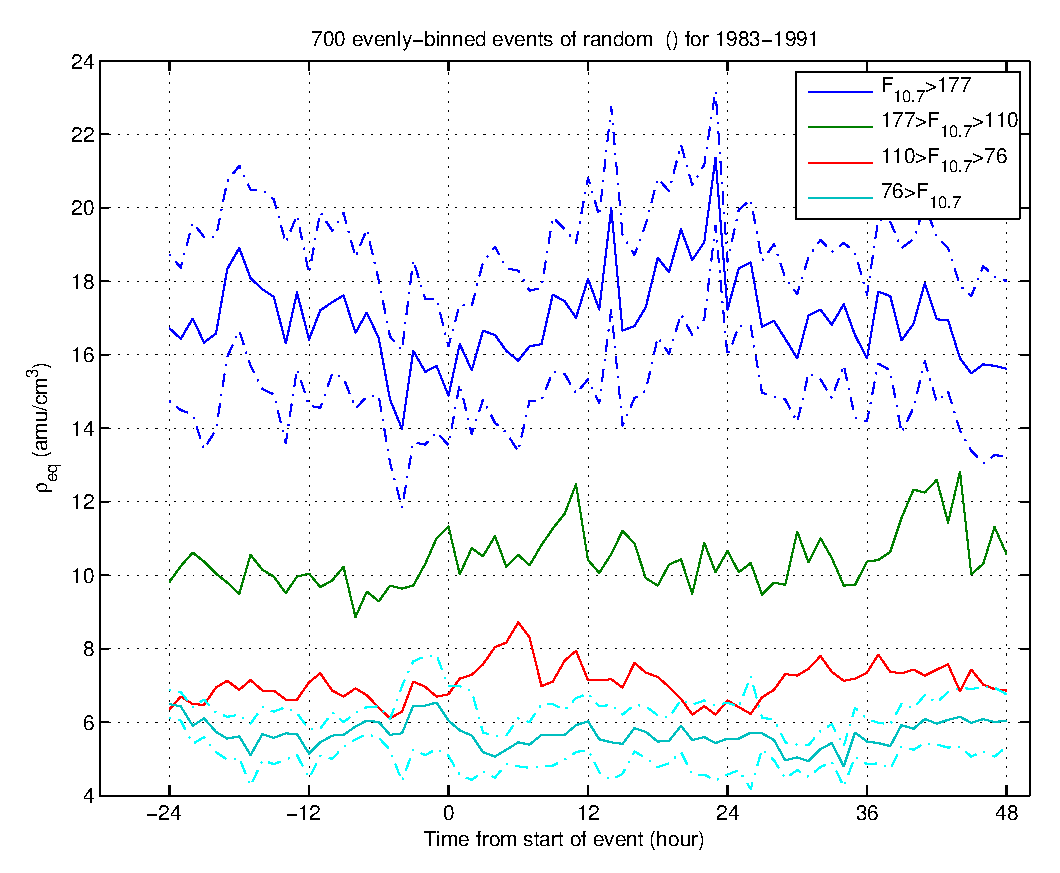
\includegraphics[scale=0.45]{paperfigures/HighLowF107rhoeq-random.eps}
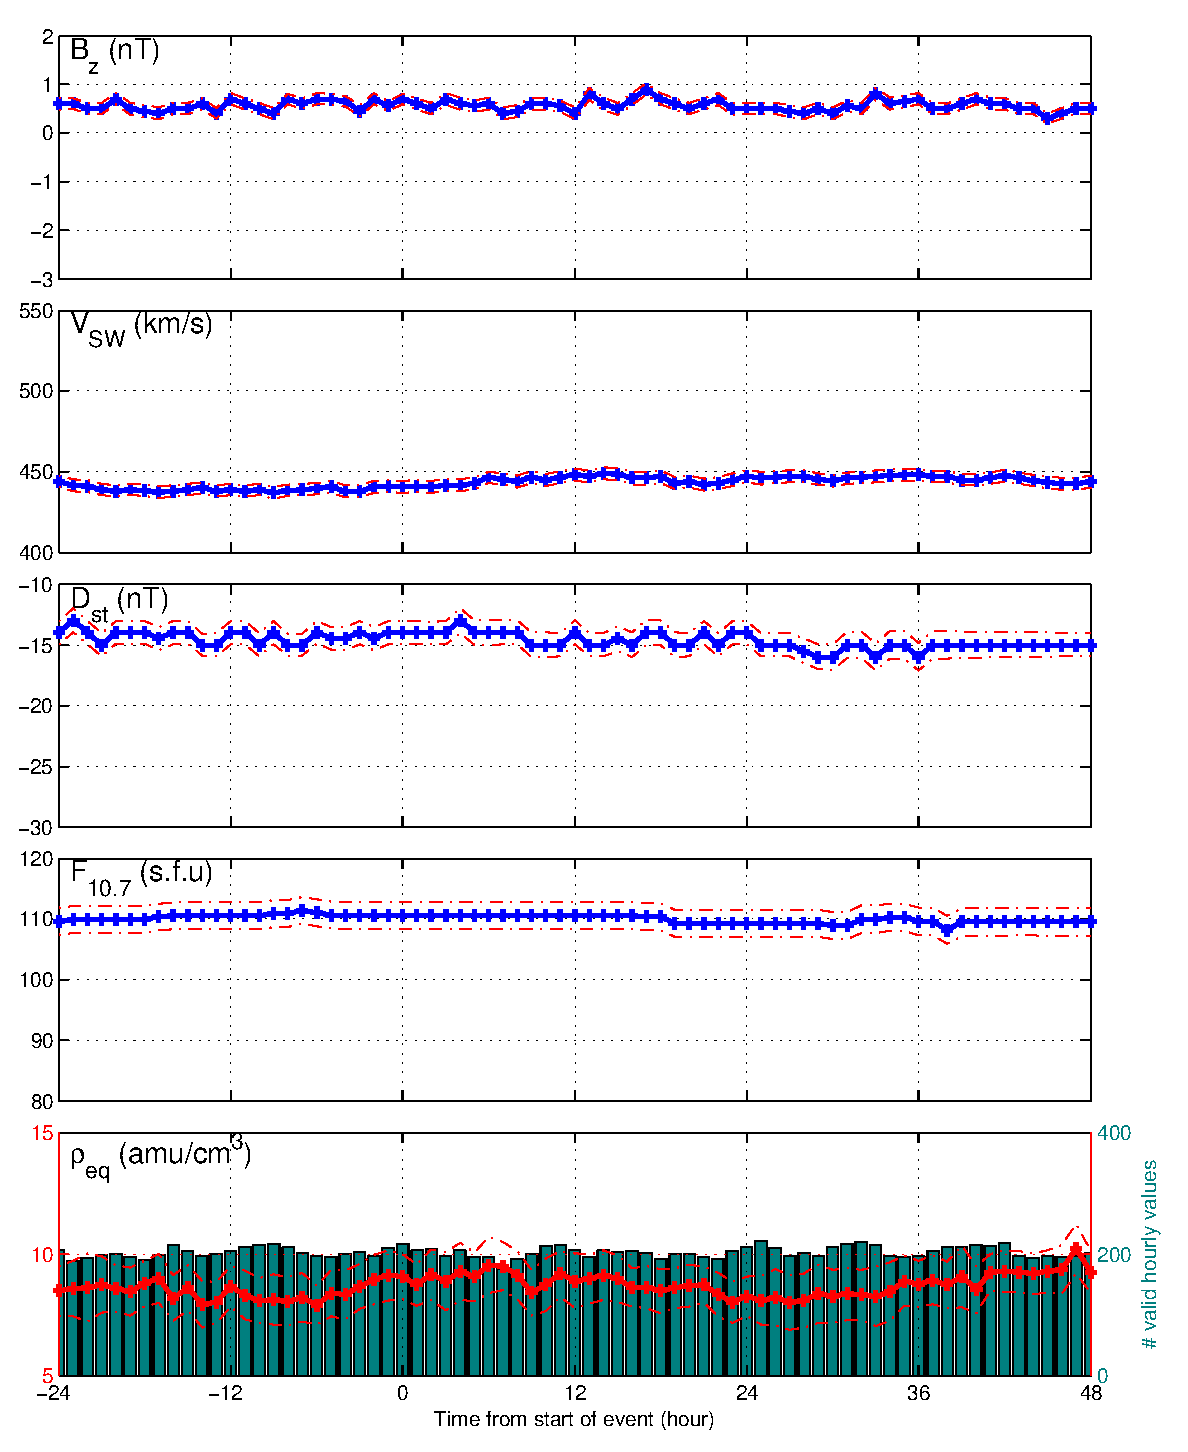
\includegraphics[scale=0.45]{paperfigures/stormavs-random.eps}
\caption{Top: $\rho_{eq}$ binned by $F_{10.7}$ for randomly selected times. Bottom: averages of randomly selected times}
\end{figure}

\begin{figure}[htp!]
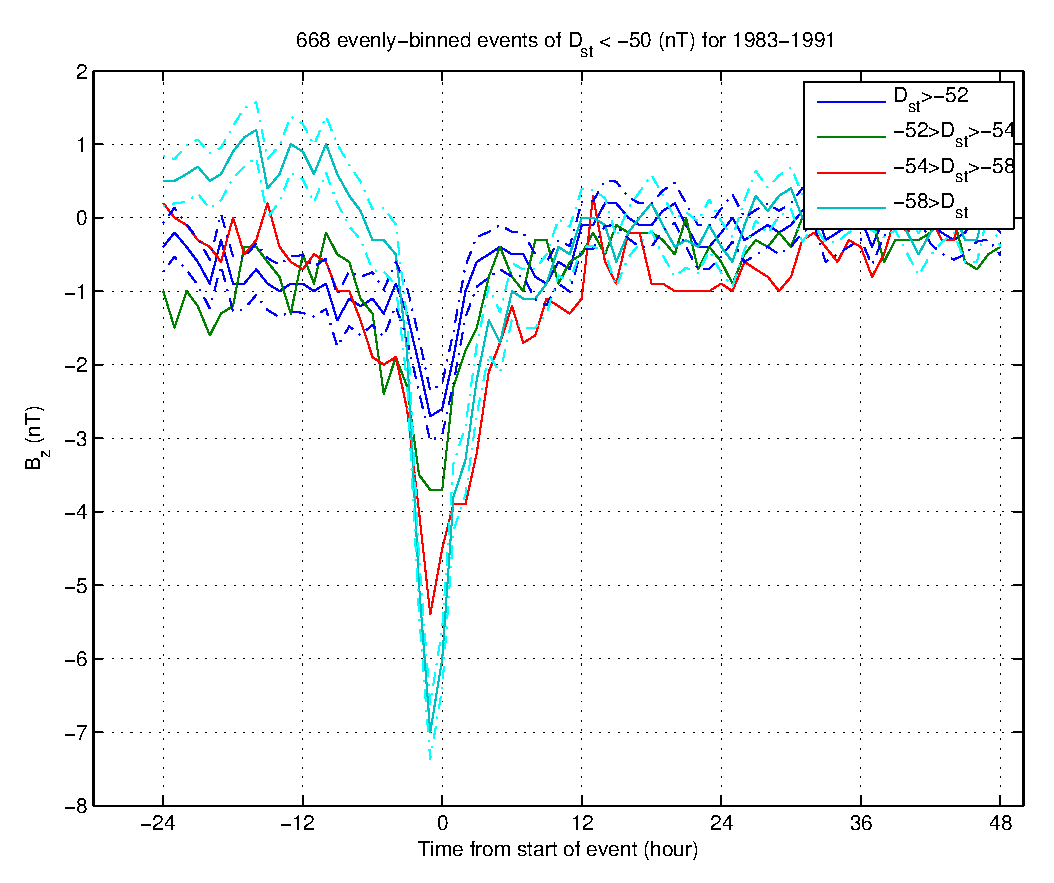
\includegraphics[scale=0.45]{paperfigures/HighLowDstBz-Dst50.eps}
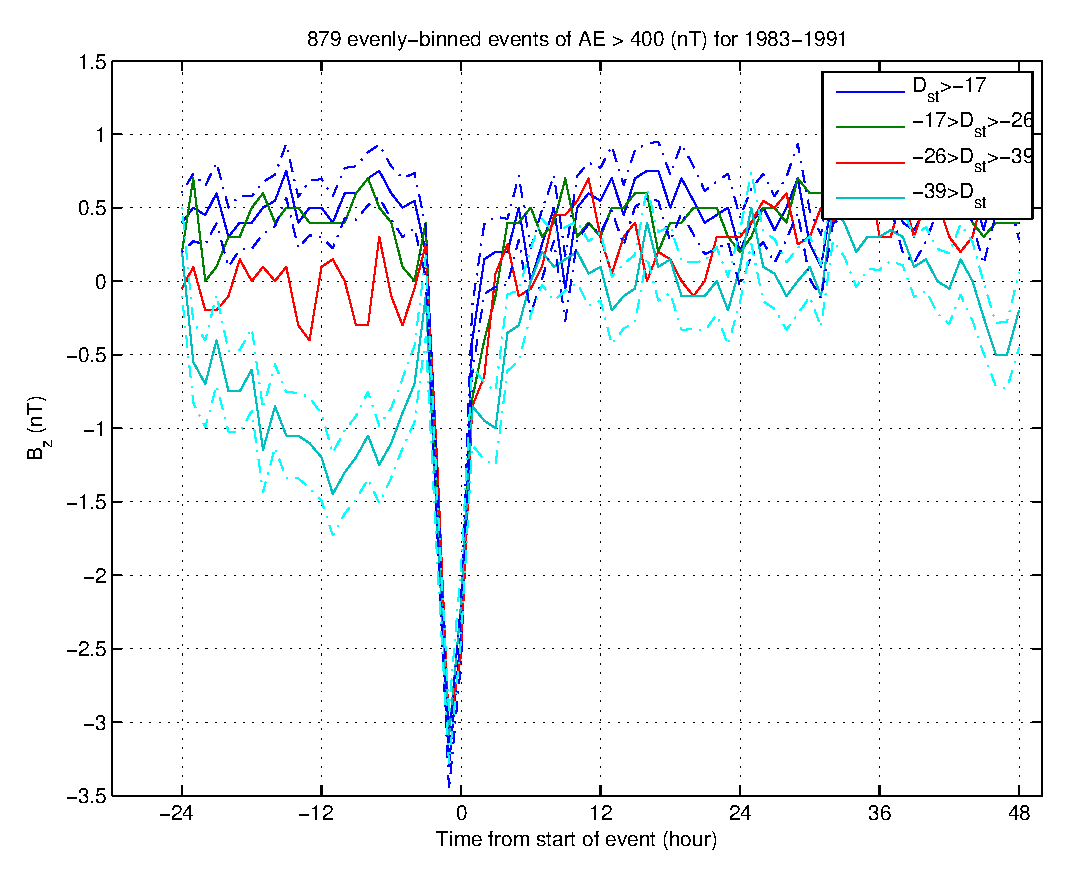
\includegraphics[scale=0.45]{paperfigures/HighLowDstBz-AE400.eps}
\caption{Top: $B_z$ binned by $D_{st}$ for $D_{st} < -50$ nT events. Bottom: $B_z$ binned by $D_{st}$ for $AE > 400$ nT events}
\end{figure}
\clearpage

\begin{figure}[htp!]
\includegraphics[scale=0.45]{paperfigures/rhoMLT.eps}
\includegraphics[scale=0.45]{paperfigures/rhoLT.eps}
\caption{Median $\rho_{eq}$ vs magnetic local time and universal time}
\end{figure}

\begin{figure}[htp!]
\includegraphics[scale=0.45]{paperfigures/DstLT.eps}
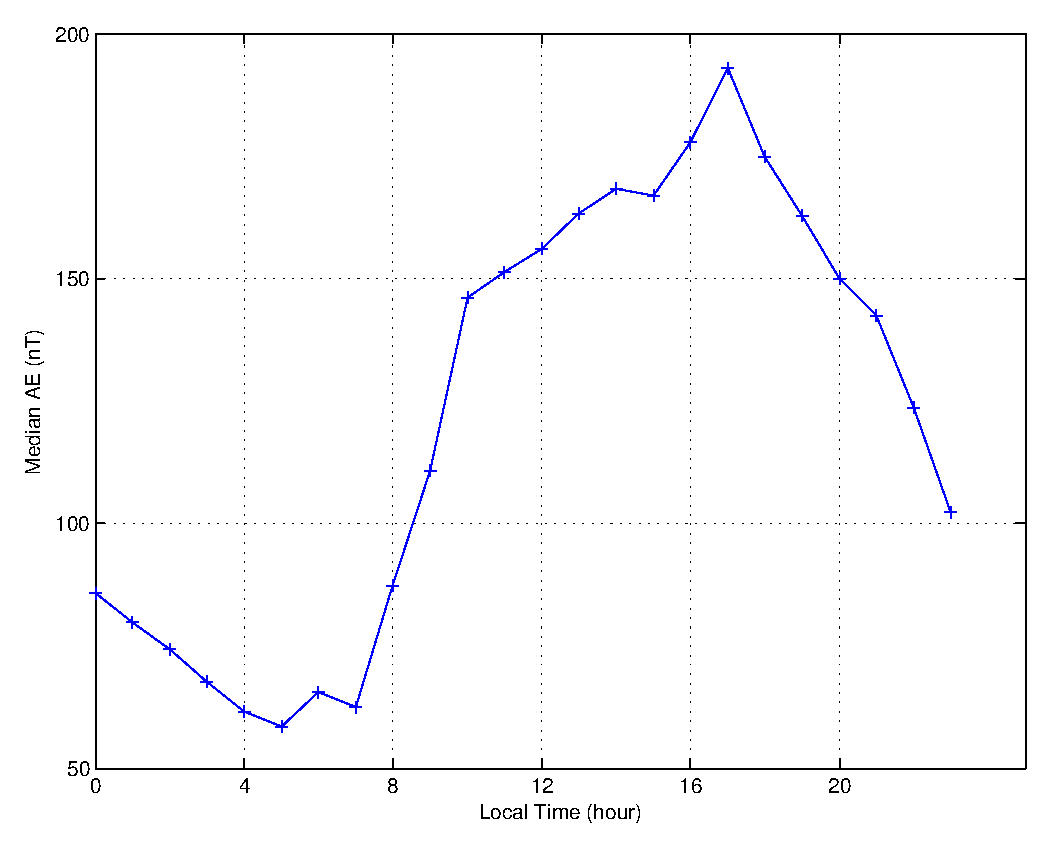
\includegraphics[scale=0.45]{paperfigures/AELT.eps}
\caption{Median $D_{st}$ vs universal time, and median AE vs universal time}
\end{figure}
\clearpage





\end{document}
